\documentclass[dvipsnames, aspectratio=169]{beamer}
\usetheme{CambridgeUS}
\usecolortheme{beaver}
\usepackage{graphicx}
\usepackage{cite}
\usepackage{bibentry}
\usepackage{amssymb}

\title[Analysis of a NOHTFPECGPPIE]{Analysis of a Novel Open Hybrid Trilateral Flash and Partial Evaporation Cycle Geothermal Power Plant Incorporated with an Ejector (NOHTFPECGPPIE)}

\author[Francis J. Antonio]{Francis Jacinto Antonio} 

\institute[UP Diliman]{Dissertation Proposal Defense}

\logo{
\includegraphics[height=1cm]{university.png}}

\date{\today}

\begin{document}
\setbeamertemplate{caption}{\raggedright\insertcaption\par}

\begin{frame}
	\maketitle
\end{frame}

\begin{frame}{Outline}
	\tableofcontents
\end{frame}

\section{Brief Introduction of NOHTFPECGPPIE}
\begin{frame}{\small Schematic Diagram Novel Open Hybrid Trilateral Flash and Partial Evaporation Cycle Geothermal Power Plant Incorporated with an Ejector (NOHTFPECGPPIE)}
	\begin{figure}[h]
    \centering
    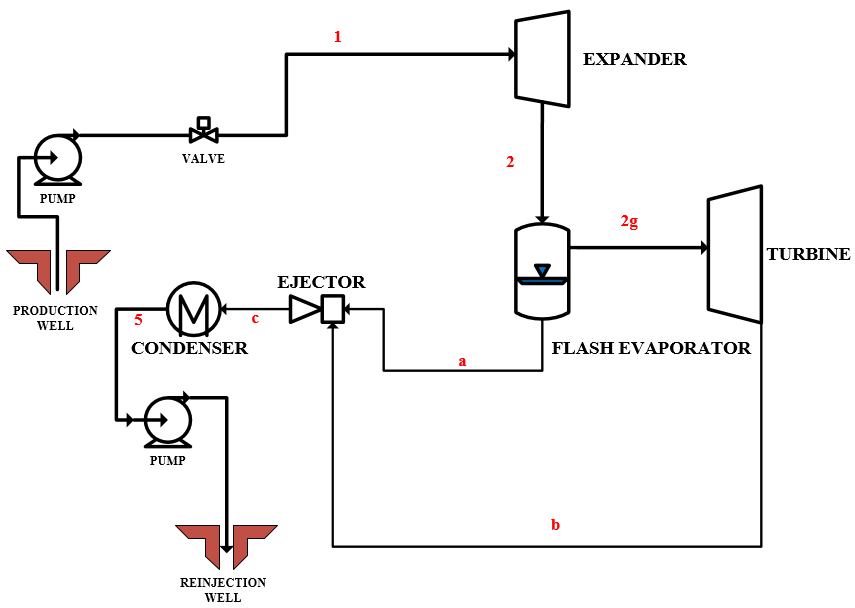
\includegraphics[height=5.25cm]{images/NOHTFPECGPPIE.PNG}
    \label{fig:NOHTFPECGPPIE}
\end{figure}
\end{frame}

\section{Introduction}
\begin{frame}{Total Final World Energy Consumption}
	\begin{table}
		\centering
		\caption{Sector Percentage Shares of Balance Factors by Forman et al. \cite{forman2016estimating}}
		\begin{tabular}{cccc}
			\hline
			Sectors & Energy Service & Exhausts/Effluents & Other Losses\\
			\hline
			World & 28 & 52 & 20\\
			Electricity & 39 & 49 & 12\\
			Industrial & 49 & 30 & 21\\
			Commercial & 40 & 33 & 27\\
			Residential & 51 & 35 & 14\\
			Transportation & 19 & 59 & 22\\
			\hline
		\end{tabular}
	\end{table}
\end{frame}

\begin{frame}{IEA 2018 World Energy Balance}\label{worldenergybal}
	\begin{table}
		\centering
		\caption{2018 IEA World Energy Balance\cite{iea2018world}}
		 \begin{tabular}{ccc}
		 \hline
		 Sectors & Sector Percentage Share & Percent Losses\\
		\hline
		Electricity & 48.19 & 51.81 \\
		Industrial & 28.56 & --- \\
		Transportation & 29.09 & ---\\
		Non-energy & 9.24 & ---\\
		Other & 33.11 & --- \\
		\hline
		\end{tabular}
	\end{table}
\end{frame}

\begin{frame}{IEA 2018 Philippine Energy Balance}
	\begin{table}
		\centering
		\caption{2018 IEA Philippine Energy Balance\cite{IEA2018PhilippineEnergyBalance}}
		 \begin{tabular}{ccc}
		 \hline
		 Sectors & Sector Percentage Share & Percent Losses\\
		\hline
		Electricity & 29.24 & 70.76 \\
		Industrial & 22.55 & --- \\
		Transportation & 36.33 & ---\\
		Non-energy & 3.72 & ---\\
		Other & 37.39 & --- \\
		\hline
		\end{tabular}
	\end{table}
\end{frame}

\begin{frame}{DOE 2017 Philippines Energy Balance}
   \begin{table}
		\centering
		\caption{\centering 2017 Department of Energy (DOE) Total Final Energy Consumption by Sector Percentage Shares\cite{doe2017energysituationer}}
		 \begin{tabular}{cc}
			 \hline
			 Sectors & Percentage Shares \\
			 \hline
			 Transportation & 34.9 \\
			 Residential & 27.1 \\
			 Industrial & 23.5 \\
		     Commercial & 13.0 \\
			 Agriculture, Fishery and Forestry & 1.5 \\
			\hline
		  \end{tabular}
	\end{table}
\end{frame}

\begin{frame}{Sectoral Shares of Waste Heat Distribution}
	\begin{table}
		\centering
		\caption{\centering Percent Sectoral Shares of Waste Heat Distribution through Waste Heat Temperatures of $<100^{\circ}C$, $100-299^{\circ}C$ and $\geq300^{\circ}C$ by Forman et al. \cite{forman2016estimating}}
		\begin{tabular}{cccc}
			\hline
			Sectors & $<100^{\circ}C$ & $100-299^{\circ}C$ & $\geq300^{\circ}C$\\
			\hline
			World & 63 & 16 & 21\\
			Electricity & 88 & 12 & 0\\
			Industrial & 42 & 20 & 38\\
			Commercial & 59 & 5 & 36\\
			Residential & 36 & 64 & 0\\
			Transportation & 46 & 54 & 0\\
			\hline
		\end{tabular}
	\end{table}
\end{frame}

\begin{frame}{Sectoral Shares of Exergy Distribution}
	\begin{table}
		\centering
		\caption{\centering Percent Sectoral Shares of Exergy Distribution through Waste Heat Temperatures of $<100^{\circ}C$, $100-299^{\circ}C$ and $\geq300^{\circ}C$  by Forman et al. \cite{forman2016estimating}}
		\begin{tabular}{cccc}
			\hline
			Sectors & $<100^{\circ}C$ & $100-299^{\circ}C$ & $\geq300^{\circ}C$\\
			\hline
			World & 21 & 24 & 55\\
			Electricity & 35 & 65 & 0\\
			Industrial & 17 & 20 & 63\\
			Commercial & 22 & 8 & 70\\
			Residential & 16 & 84 & 0\\
			Transportation & 22 & 78 & 0\\
			\hline
		\end{tabular}
	\end{table}
\end{frame}

\begin{frame}{Heat Sources: 3 Thermal Stratification\cite{jouhara2018waste}}
		\begin{alertblock}{Low-Thermal Grade (Low-Enthalpy Grade)}
			Heat sources below $200^{\circ}Celsius$
		\end{alertblock}
	
		\begin{block}{Medium-Thermal Grade}
			Heat sources ranging from $200-400^{\circ}Celsius$
		\end{block}
		
		\begin{block}{High-Thermal Grade}
			Heat sources above $400^{\circ}Celsius$
		\end{block}	
\end{frame}

\begin{frame}{Low-Grade Thermal Sources: Exhaust Gas Temperature Range in Different  Thermal Processes by Bruckner et al\cite{bruckner2015industrial}}
    \begin{table}[]
        \centering
        \begin{tabular}{p{7.5cm}p{2.5cm}}
        \hline
        \textbf{Thermal Processes} &
        \textbf{Temp. Range ($^{\circ}C$)} \\
        \hline
     Exhaust gases exiting recovery devices in gas-fired boilers, ethylene furnaces, etc. &  70 - 230 \\
     Process steam condensate & 50 - 90 \\
     Cooling water from furnace doors & 30 - 50 \\
     Cooling water from annealing furnaces & 70 - 230 \\
     Cooling water from air compressors & 30 - 50 \\
     Cooling water from internal combustion engines & 70 - 120 \\
     Cooling water from air conditioning and refrigeration condensers & 30-40 \\
     Drying, baking, and curing ovens & 90 - 230 \\
     Hot processed liquids & 30 - 230 \\
     \hline
    \end{tabular}
    \end{table}
\end{frame}

\begin{frame}{Process Industries that have Low-Grade Thermal Sources by Bruckner et. al\cite{bruckner2015industrial}}
    \begin{columns}
        \column{0.45\textwidth}
		\begin{block}{Food and Beverage}
			Cleaning, Cooking, Pasteurizing, Whitening, Drying, Washing, Sterilizing, Boiling, Heat Treatment and Drainage
		\end{block}
		
		\begin{block}{Textile}
			Dry Heating, Ironing, Washing, Bleaching, Dyeing, Drying and Steaming
		\end{block}
		
		\begin{block}{Paper}
			Pulp and Paper Drying
		\end{block}
		
		\column{0.45\textwidth}
		\begin{block}{Chemical Process}
			Boiling, Distilling, and Various Chemical Processes
		\end{block}
		
		\begin{block}{Other Process Industries}
			Non-metallic mineral processes, Wood drying, Metal Cleaning and Paint Drying
		\end{block}
	\end{columns}
\end{frame}

\begin{frame}{Waste Recovery Technologies that uses Low Grade Thermal Sources\cite{jouhara2018waste}}
    \begin{enumerate}
        \item Economizer
        \item Rotary Regenerator
        \item Heat Pumps
        \item Recuperators
        \item Thermo Photovoltaic Generators
        \item Piezoelectric Power Generation
    \end{enumerate}
\end{frame}

\begin{frame}{2017 World Energy Council (WEC): World Energy Resources: Geothermal\cite{council2017world,WorldEnergyCouncil2013}}
\begin{itemize}
    \item Low-temperature geothermal resources in the world is about 140 EJ/yr of heat.
    \item World energy consumption is now about 420 EJ/yr.
\end{itemize}
$ 1 Exajoule (EJ) = 1 x 10^{8} Joules (J) = 2.778 x 10^{11} kW-hr$
\end{frame}

\begin{frame}{Geothermal Resource Type (GRT)\cite{white1975assessment}}
\begin{columns}
    \column{0.6\textwidth}
    \begin{enumerate}
        \item Convective Hydrothermal Resources 
            \begin{itemize}
                \item Vapor Dominated (VD)
                \item Liquid Dominated (LD)
            \end{itemize}
        \item Other Hydrothermal Resources 
            \begin{itemize}
                \item Sedimentary basin (SB)
                \item Geopressured (GP)
                \item Radiogenic (R)
            \end{itemize}
        \item Hot Rock Resources 
            \begin{itemize}
                \item Solidified or Hot-Dry Rock (HDR)
                \item Part Still Molten or Magma
            \end{itemize}
    \end{enumerate}
    \column{0.5\textwidth}
       \begin{table}
		\centering
		 \begin{tabular}{p{1cm}p{1.5cm}}
			 \hline
			 GRT & Temperature Range $^{\circ}C$ \\
			 \hline
			 VD & $\approx240$ \\
			 LD & 20-350 \\
			 SB & 20-150 \\
		     GP & 90-200 \\
			 R & 30-150 \\
			 HDR & 90-650 \\
			 Magma & $>600$\\
			\hline
		  \end{tabular}
	\end{table}
\end{columns}
\end{frame}

\begin{frame}{GRT: Convective Hydrothermal Resources:VD\cite{WorldEnergyCouncil2013}}
\begin{columns}
    \column{0.45\textwidth}
    \begin{figure}
        \centering
        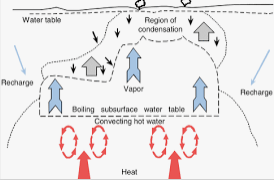
\includegraphics[height=4cm]{images/VDregion.png}
        \caption{\centering \scriptsize Vapor Dominated Resource\cite{lund2015worldwide}}
        \label{fig:vdr}
    \end{figure}
    \column{0.45\textwidth}
    \begin{figure}
        \centering
        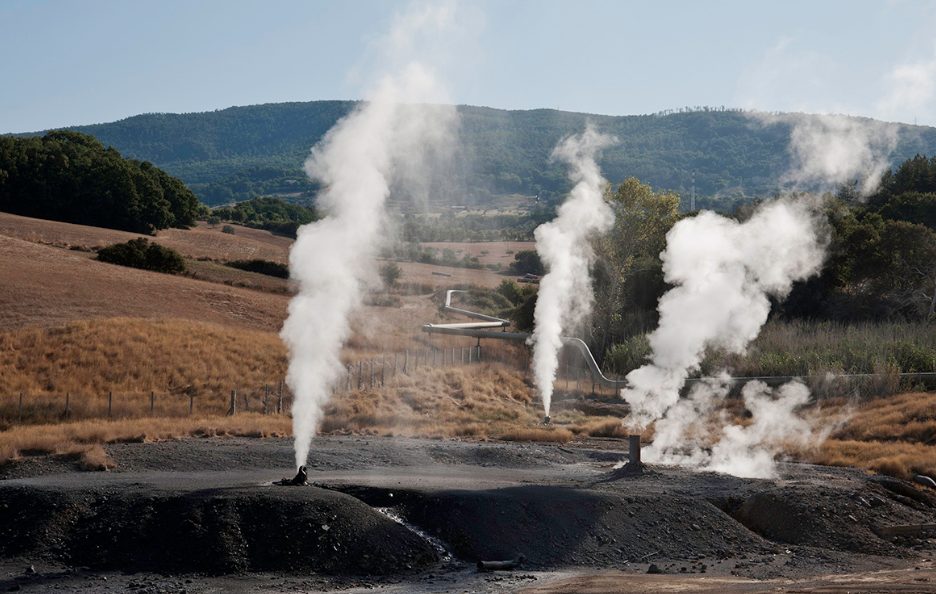
\includegraphics[height=2cm]{images/Lardello Italy.png}
        \caption{\centering \tiny Geysers at Larderello,Italy\cite{PaoloCagnacciPhotography}}
        \label{fig:larderello}
    \end{figure}
    \begin{figure}
        \centering
        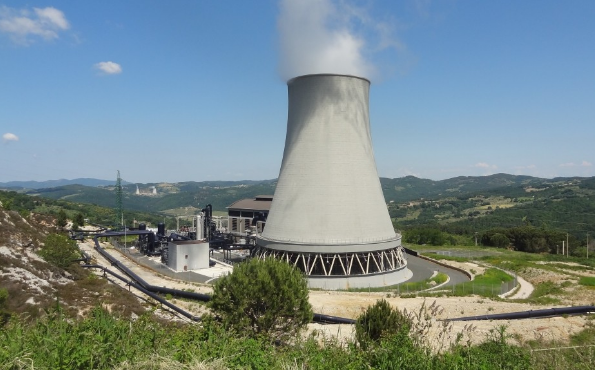
\includegraphics[height=2cm]{images/LarderelloGPP.png}
        \caption{\centering \tiny Sasso 2 geothermal plant by Enel Green Power, Tuscany, Italy (source: Volcanex)\cite{LarderelloGPP}}
        \label{fig:larderellogpp}
    \end{figure}
\end{columns}
\end{frame}

\begin{frame}{Power Station Energy Shares: Philippines}
   \begin{table}[h]
		\centering
		\caption{\centering 2018 IEA Phlippine Energy Balance - Power station energy shares\cite{IEA2018PhilippineEnergyBalance}}
		\label{tab:phppowerstationenergyshares}
		 \begin{tabular}{ccc}
			 \hline
			 Source of Energy & Percent Shares to Power Station \\
			 \hline
			 Oil Products & 2.50 \\
			 Coal & 51.06 \\
			 Natural Gas & 11.48 \\
		     Biofuels and Waste & 0.72 \\
			 \textbf{Geothermal} & \textbf{30.74} \\
			 Solar/Wind/Tide & 0.72 \\
			 Hydro & 2.78\\
			\hline
			Total & 100\% \\
			\hline
		  \end{tabular}
    \end{table}
\end{frame}

\begin{frame}{Geothermal Projected Capacities: Top Five Geothermal Power Producing Countries \cite{irenageothermalpower2017}}
    \begin{table}[h]
		\centering
		\caption{\centering Projected Geothermal Capacity (MW) for the Year 2016, 2025, and $>$2025}
		\label{tab:projectedgeothermalpower}
		\begin{tabular}{cccc}
			\hline
			 & 2016 & 2025 & $>$2025**\\
			\hline
			USA & 3490.3 & 3874.3 & 5425.3\\
			Indonesia & 1468.9 & 3410.7 & 4270.2\\
			\textbf{Philippines} & \textbf{1943.4} & \textbf{2104.4} & \textbf{2834.4}\\
			New Zealand & 1058.8 & 1128.8 & 1483.8\\
			Iceland& 612.4 & 752.4 & 1322.4\\
			\hline
		\end{tabular}
		\caption{\centering** Capacity additions after 2025 correspond to planned and deferred projects without completion date}
	\end{table}
\end{frame}

\begin{frame}{DOE Project: Detailed Assessment of Selected Low Enthalpy Geothermal
Resources in the Philippines\cite{halcon2015detailed}}
    \begin{alertblock}{Primary Objective}
        Accelerate the development of  of Low to Medium
        Enthalpy Geothermal Resource Area, with a temperature ranging from 90$^{\circ}$C - 150$^{\circ}$C, mainly for power generation.
    \end{alertblock}
    \begin{block}{Secondary Objectives}
         Assessment and realization of the economic feasibility of small scale geothermal power projects for local power needs.
    \end{block}
    \begin{block}{Secondary Objectives}
        Prepares of a comprehensive data package that will showcase this type of geothermal resource for future private investors.
    \end{block}
\end{frame}

\begin{frame}{DOE Project: Detailed Assessment of Selected Low Enthalpy Geothermal
Resources in the Philippines\cite{halcon2015detailed}}
    \begin{block}{Identified Low Enthalpy Gesource Resource Areas}
        Banton Island, Romblon
    \end{block}
    \begin{figure}
        \centering
        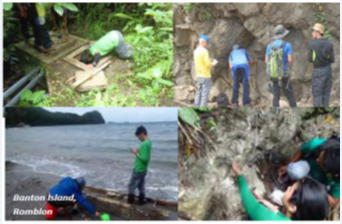
\includegraphics[height=2.5cm]{images/DOEbontonisland.PNG}
        \caption{\centering Conducting Geological, Geochemical and Controlled Surface Magneto Telluric (CSMT) Survey at Banton Island, Romblon}
    \end{figure}
\end{frame}

\begin{frame}{DOE Project: Detailed Assessment of Selected Low Enthalpy Geothermal
Resources in the Philippines\cite{halcon2015detailed}}
    \begin{block}{Identified Low Enthalpy Gesource Resource Areas}
        Maricaban (Tingloy) Island, Batangas (left figure) \\
        Balut Island, Davao del Sur (right figure)
    \end{block}
    \begin{figure}
        \centering
        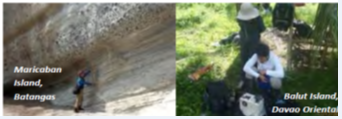
\includegraphics[height=2.5cm]{images/DOEmaricaban.PNG}
        \caption{\centering \small Conducting Geological, Geochemical and CSMT Survey at Maricaban (Tingloy Island), Batangas and Balut Island, Davao Oriental}
    \end{figure}
\end{frame}

\begin{frame}{Tingloy Island Geothermal Wells}
    \begin{columns}
    \column{0.45\textwidth}
    \begin{table}[h]
        \centering
        \caption{Tingloy Geothermal Well Data}
        \begin{tabular}{ccc}
        \hline
            Slim Well &  Type of Well & Depth (m) \\
            \hline
             SH01 & Production & 490-500 \\
             SH02 & Reinjection & 1000-1015 \\
             \hline
        \end{tabular}
        \label{tingloywells}
    \end{table}
    \begin{table}[h]
        \centering
        \begin{tabular}{cp{2cm}p{1.75cm}}
        \hline
            Slim Well & Wellhead Pressure (kPa) & Wellhead Temperature ($^\circ$C)\\
            \hline
             SH01 & 4,820-4,860 & 120-130 \\
             SH02 & 9,600-9,610 & 130-140 \\
             \hline
        \end{tabular}
    \end{table}
    \column{0.45\textwidth}
    \begin{figure}
        \centering
        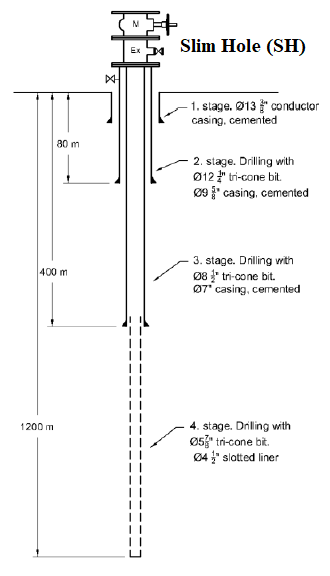
\includegraphics[height=4cm]{images/slimhole1.png}
        \caption{\centering Slim Wells used for Production and Reinjection Wells \cite{thorhallsson2012slim}}
        \label{fig:slimwells}
    \end{figure}
    \end{columns}
\end{frame}

\begin{frame}{NOHTFPECGPPIE Geothermal Wells using Tingloy Data from DOE\cite{halcon2015detailed}}
    \begin{figure}
        \centering
        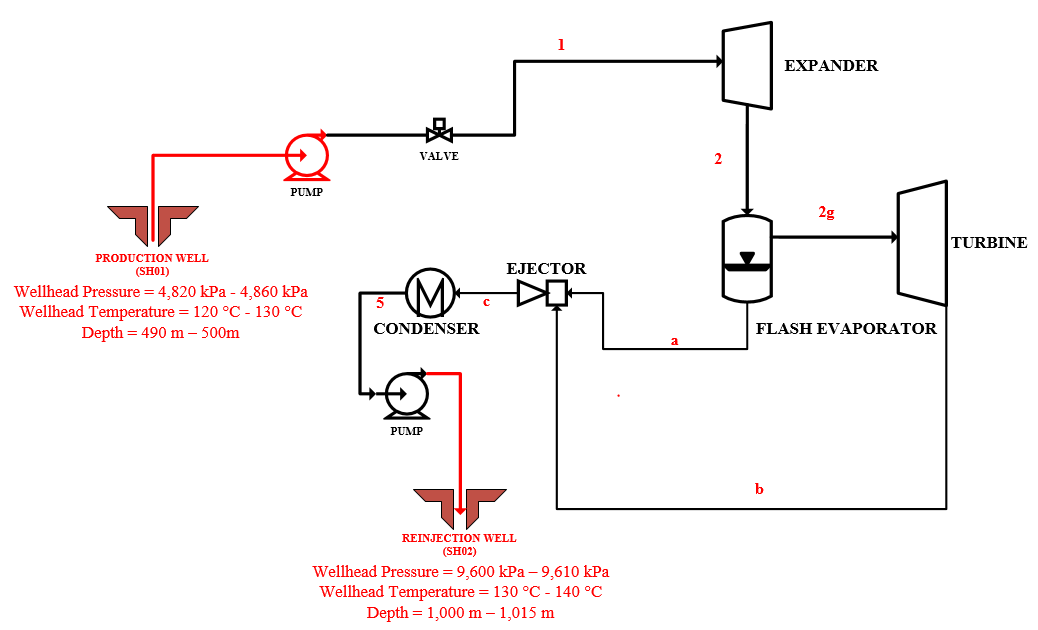
\includegraphics[height=0.4\textwidth]{images/nohtfpecgppiewells.png}
    \end{figure}
\end{frame}

\begin{frame}{Tingloy Geothermal Well Brine Density Readings for SH01 - First Test\cite{halcon2015detailed}}
    \begin{columns}
    \column{0.45\textwidth}
    \begin{figure}
        \centering
        \caption{\centering First Run Down Test}
        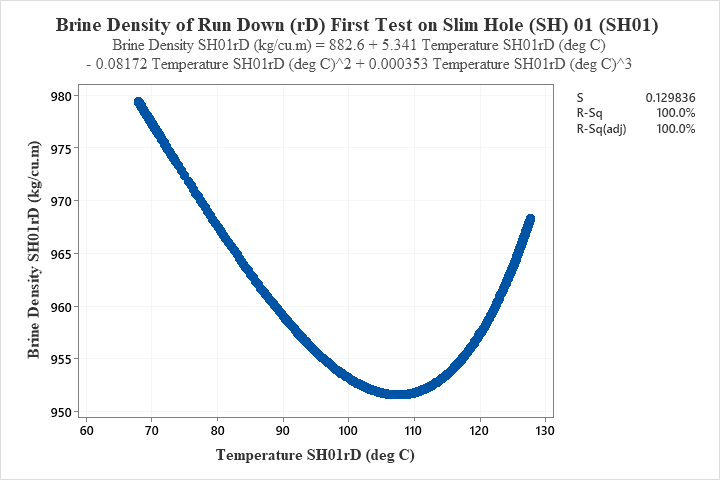
\includegraphics[height=4cm]{images/sh01r1d.png}
    \end{figure}
    \column{0.45\textwidth}
    \begin{figure}
        \centering
        \caption{\centering First Run Up Test}
        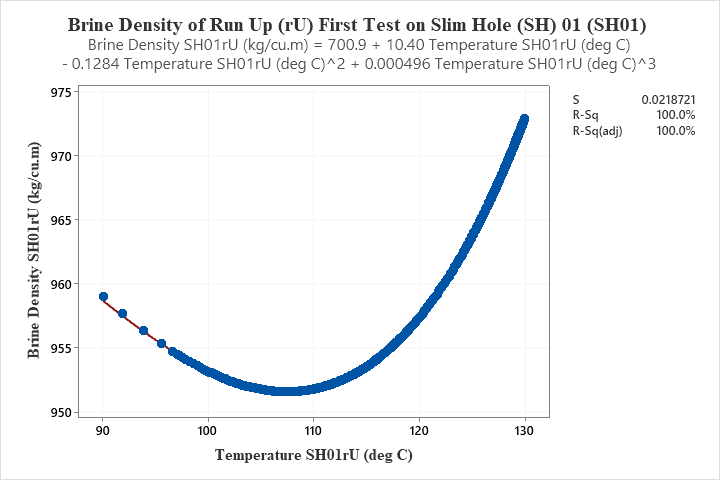
\includegraphics[height=4cm]{images/sh01r1u.png}
    \end{figure}
    \end{columns}
\end{frame}

\begin{frame}{Tingloy Geothermal Well Brine Density Readings for SH01 - 2nd Test\cite{halcon2015detailed}}
    \begin{columns}
    \column{0.45\textwidth}
    \begin{figure}
        \centering
        \caption{\centering Second Run Down Test}
        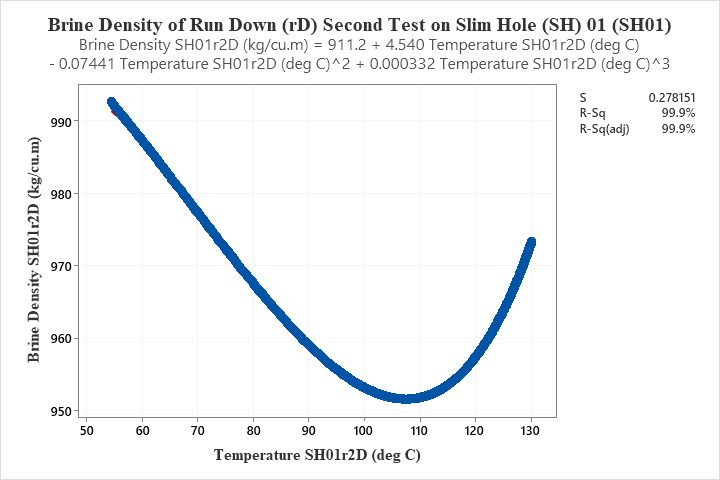
\includegraphics[height=4cm]{images/sh01r2d.png}
    \end{figure}
    \column{0.45\textwidth}
    \begin{figure}
        \centering
        \caption{\centering Second Run Up Test}
        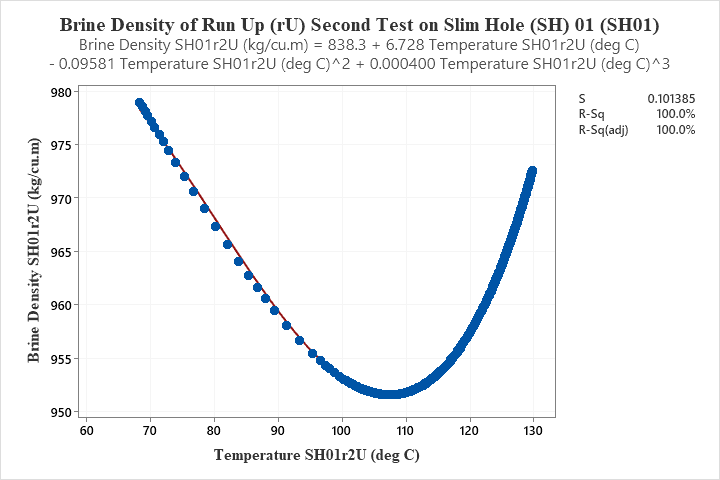
\includegraphics[height=4cm]{images/sh01r2u.png}
    \end{figure}
    \end{columns}
\end{frame}

\begin{frame}{Tingloy Geothermal Well Brine Density Readings for SH01 - 3rd Test\cite{halcon2015detailed}}
    \begin{columns}
    \column{0.45\textwidth}
    \begin{figure}
        \centering
        \caption{\centering Third Run Down Test}
        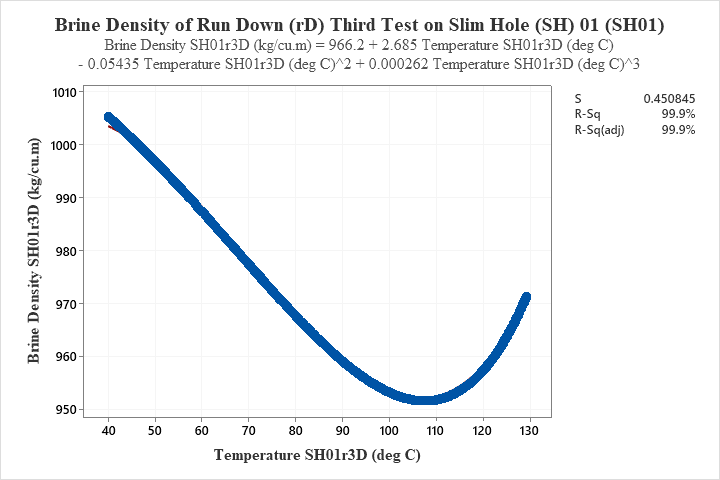
\includegraphics[height=4cm]{images/sh01r3d.png}
    \end{figure}
    \column{0.45\textwidth}
    \begin{figure}
        \centering
        \caption{\centering Third Run Up Test}
        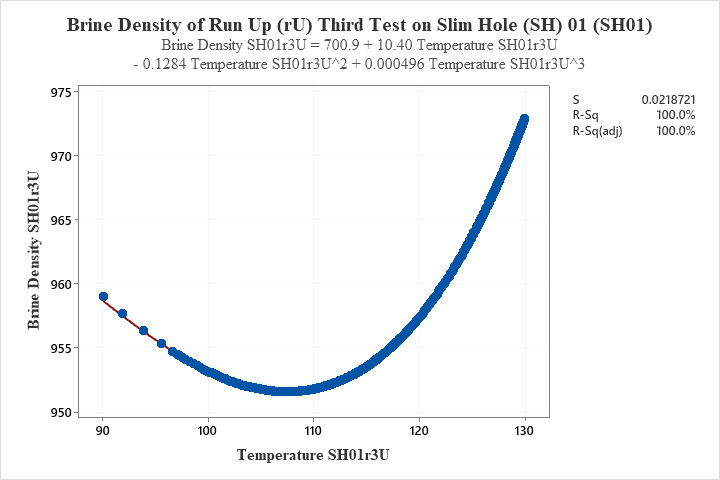
\includegraphics[height=4cm]{images/sh01r3u.png}
    \end{figure}
    \end{columns}
\end{frame}

\begin{frame}{Types of Expansion Devices Based on Working Principles\cite{smith2014power}}
   \begin{columns}
   \column{0.45\textwidth}
   \begin{enumerate}
        \item Turbine or Turbo Expanders
            \begin{itemize}
                \item Radial Inflow
                \item Radial Outflow
                \item Axial
            \end{itemize}
        \item Positive Displacement
            \begin{itemize}
                \item Scroll
                \item Screw
                \item Rotary Vane
                  \begin{itemize}
                    \item Wankel
                  \end{itemize}
                \item Piston
                \item Roots
            \end{itemize}
        \item Ejector
    \end{enumerate}
    \column{0.45\textwidth}
    \begin{figure}
        \centering
        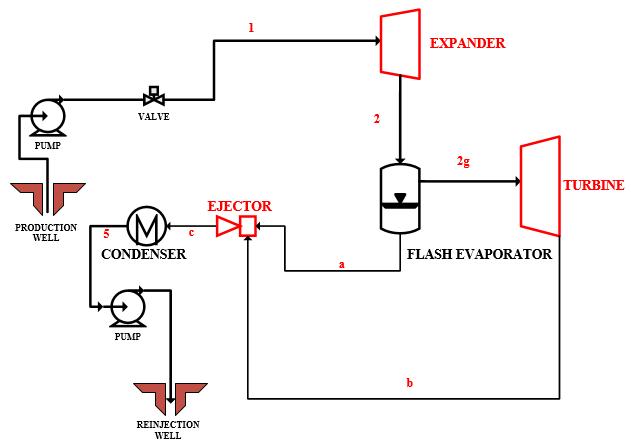
\includegraphics[height=4.5cm]{images/nohtfpecgppiexd.png}
        \caption{\centering \scriptsize NOHTFPECGPPIE emphasizing expansion devices}
    \end{figure}
   \end{columns}
\end{frame}

\begin{frame}{Expander}
	\begin{table}[h]
		\centering
		\caption{\centering Capacity Ranges, Rotative Speeds and Costs of the Different Types of Expander Installed in an Organic Rankine Cycle\cite{pethurajan2018issues}}
		\label{tab:expandercapacityinORC}
		\begin{tabular}{|p{3.75cm}|p{2cm}|p{2.5cm}|p{1.5cm}|}
			\hline
			Type & Capacity Range (kW) & Rotative Speed (rpm) & Cost\\
			\hline
			Radial-Inflow Turbine & 50-500 & 8,000-80,0000 & High\\
			Scroll Expander & 1-10 & $<6,000$ & Low\\
			Screw Expander & 15-200 & $<6,000$ & Medium\\
			Rotary Vane Expander & 1-10 & $<6,000$ & Low\\
			\hline
		\end{tabular}
	\end{table}
\end{frame}

\begin{frame}{Expander}
    \begin{table}[h]
		\centering
		\caption{\centering Advantages and Disadvantages of the Different Types of Expander Installed in an Organic Rankine Cycle\cite{pethurajan2018issues}}
		\label{tab:expanderadvanddisadvinorc}
		\begin{tabular}{p{3cm}p{3.5cm}p{3.5cm}}
			\hline
			Type & Advantages & Disadvantages\\
			\hline
			Radial-Inflow Turbine & Lightweight with High efficiency & Cannot bear two-phase flow \\
			Scroll Expander & High efficiency, lightweight, low rotating speed and Tolerable two-phase flow & Requires lubrication and modification \\
			\hline
		\end{tabular}
	\end{table}
\end{frame}

\begin{frame}{Expander}
    \begin{table}[h]
		\centering
		\caption{\centering Advantages and Disadvantages of the Different Types of Expander Installed in an Organic Rankine Cycle\cite{pethurajan2018issues}}
		\label{tab:expanderadvanddisadvinorc}
		\begin{tabular}{p{3cm}p{3.5cm}p{3.5cm}}
			\hline
			Type & Advantages & Disadvantages\\
			\hline
			Screw Expander & Tolerable two-phase flow, low rotating speed and high efficiency & Requires lubrication \\
			Rotary Vane Expander & Tolerable two-phase flow, stable torque, simple structure, low cost and noise & Requires lubrication and low capacity \\
			\hline
		\end{tabular}
	\end{table}
\end{frame}

\begin{frame}{Scroll Expander: Operating Conditions}
    \begin{table}[h]
    \centering
    \caption{Operating Conditions of a Scroll Steam Expander\cite{kim2007scroll}}
    \label{tab:scrollexpanderopcond}
    \begin{tabular}{p{2cm}p{2.5cm}p{2.5cm}p{2.5cm}}
    \hline
        Shaft speed (rpm) & Inlet Pressure (kPa) & Outlet Pressure (kPa) & Inlet Temperature ($^{\circ}$C) \\
    \hline
         1,384 & 1,201.6 & 114.0 & 139 \\
         1,205 & 1,199.7 & 112.8 & 143 \\
         1,130 & 1,236.0 & 113.6 & 144 \\
         1,011 & 1,301.7 & 113.7 & 145 \\
    \hline
    \end{tabular}
\end{table}
\end{frame}

\begin{frame}{Selections of Steam Expander based on criteria for Low-Power Rankine Cycle\cite{badr1991expansion}}
    \begin{table}[h]
    \centering
    \label{tab:steamexpanderselection}
    \begin{tabular}{p{3cm}p{1.25cm}p{1.25cm}p{1.25cm}p{1.225cm}p{1.5cm}}
    \hline
        Targets & Turbines & R.Piston & Helical-Screw & Rotary Vane & Wankel \\
    \hline
         5-20 kW\textsuperscript{1} & No & Yes & Yes & Yes & Yes \\
        3,000-5,000 rpm\textsuperscript{2} & No & Yes & Yes & Yes & Yes \\
        $65-75\%\textsuperscript{3}$ & No & No & Yes & Yes & Yes \\
        Two-phase flow\textsuperscript{4} & No & Low & Yes & Yes & Yes \\
        Lubrication\textsuperscript{5} & --- & --- & No & Yes & No \\
    \hline
    \end{tabular}
    \caption{\scriptsize 1 = Low power output in kiloWatts, 2 = Low rotational speed in revolutions per minute (rpm), 3 = Isentropic Expander Efficiency, 4 = Ability of the expander to allow wet expansion without adverse effect on the performance and life of the expander(i.e. can handle two-phase flow expansion), 5 = Lubrication Problems during operation.}
    \end{table}
\end{frame}

\begin{frame}{Performance Map for Different Types of Expander\cite{badr1991expansion}}
\begin{figure}
    \centering
    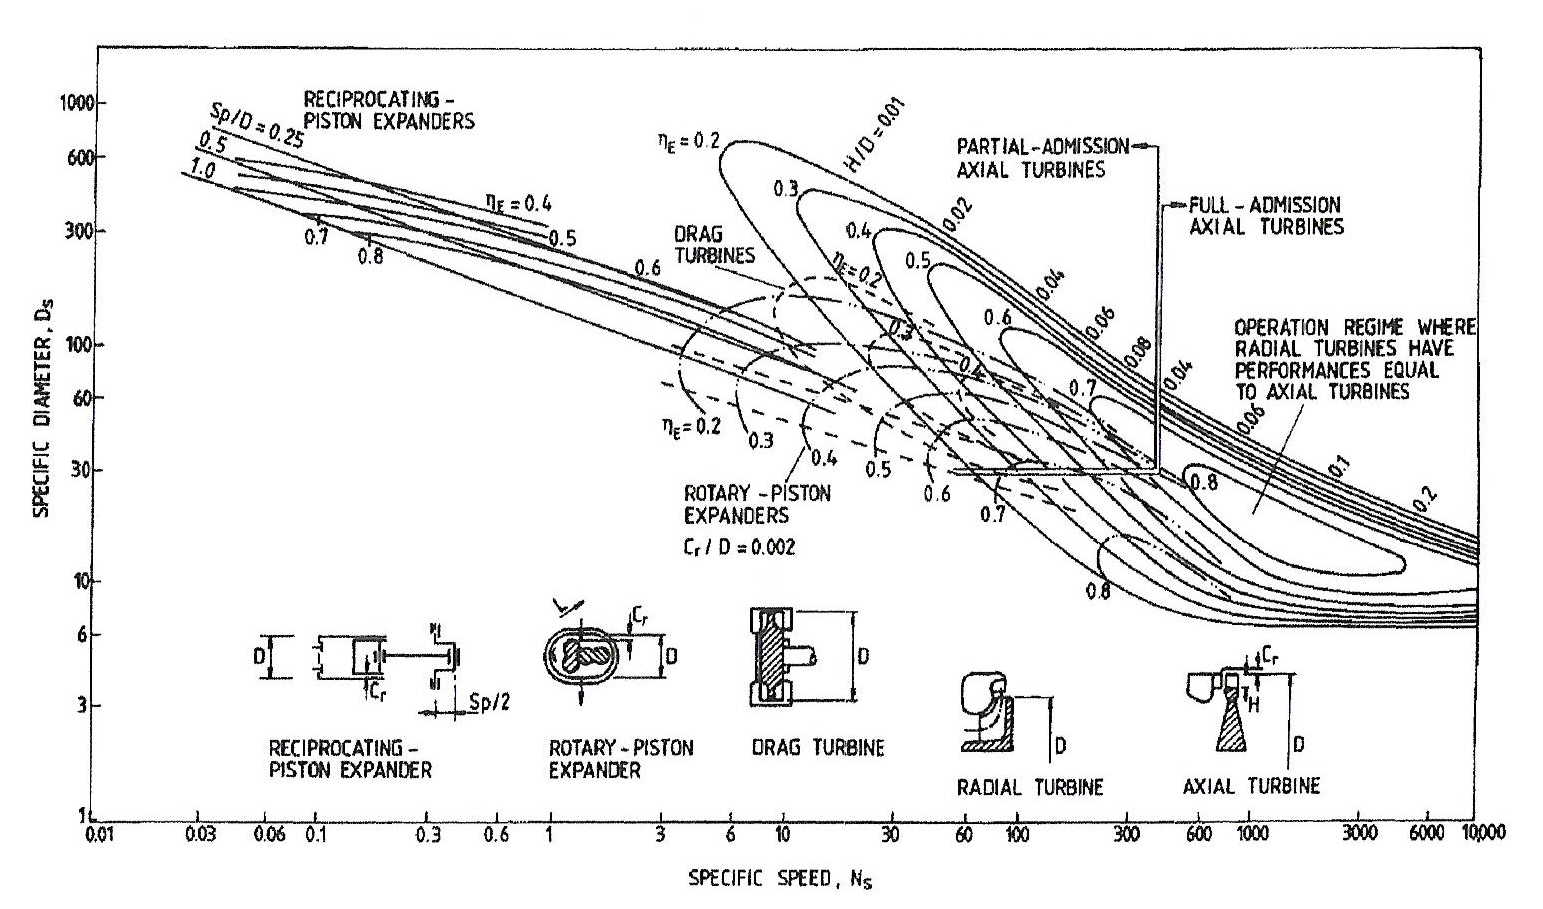
\includegraphics[height=6.25cm]{images/Expander1.png}
    \label{fig:expanderperformancetype}
\end{figure}
\end{frame}

\begin{frame}{Use of Expanders in Trilateral Flash Cycle (TFC)}
    \begin{block}{Cipollone et al. 2017 \cite{cipollone2017low}}
     \begin{itemize}
         \item Remarks: Novelty of the research is the use of \textbf{rotary positive displacement expander}
         \begin{itemize}
             \item Findings: R1234z(E) and propane provides a greater specific work, however, it would require built-in  \textbf{volume ratios of 8 and 14}, respectively, which is \textbf{beyond the capabilities of rotary positive displacement which is 5}.
         \end{itemize}
         \item Cycle: Trilateral Flash Cycle (TFC)
         \item Analysis: Thermodynamic Analysis
         \item Working Fluids: R1234yf, R1234z(E), R134a, Propane, Cyclopropane, R1234zE/CO2 (0.9/0.1), Propane/CO2 (0.9/0.1), Propane/CO2 (0.8/0.2), Propane/CO2 (0.7/0.3)
         \item Working Temperatures: Heat Source Temperature of 100$^{\circ}C$ and Heat Sink Temperature of 40$^{\circ}C$
     \end{itemize}
    \end{block}
\end{frame}

\begin{frame}{Converted Scroll Compressor into Expanders\cite{zhao2019expansion}}
    \begin{table}[h]
        \centering
        \begin{tabular}{cp{2.5cm}p{2.25cm}p{2.5cm}c}
        \hline
            Working Fluid & Output Power (kW) & Expansion Ratio & Rotational Speed (rpm) & Efficiency (\%) \\
            \hline
            R123 & 1.54 & 3.84 & 2,165 & 86 \\
            R123 & 0.75 & --- & 2,100 & 38 \\
            R245fa & 2.3 & 5.2 & 2,970 & 73 \\
            R245fa & 1.8 & 2-7 & 3,500 & 75.7 \\
            R123 & 2.78 & --- & --- & 85.17 \\
            R245fa & --- & 4.58 & 3,000 & 84.9 \\
            R245fa & 1.016 & 10.68 & 3,496 & 77.74 \\
            R123 & --- & --- & 3,000 & --- \\
            R134a & 0.557 & 3.6 & 3,450 & 78 \\
            R245fa & 3.75 & --- & 3,500 & 58 \\
            \hline
        \end{tabular}
    \end{table}
\end{frame}

\section{Review of Literature}
\begin{frame}{Trilateral Flash Closed Cycle (TFC)}
\begin{columns}
    \column{0.45\textwidth}
    \begin{figure}[h]
      \centering
      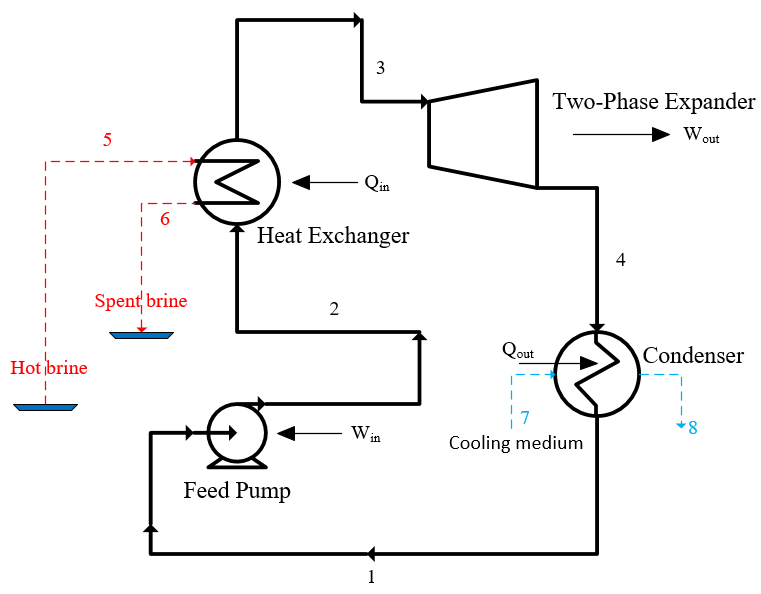
\includegraphics[height=4cm]{images/TLC.png}
      \caption{\scriptsize Schematic Diagram of an Actual Trilateral Closed Cycle (TFC) \cite{smith2014power}}
      \label{fig:tlcschematicdiagram}
   \end{figure}
   \column{0.45\textwidth}
    \begin{figure}[h]
    \centering
    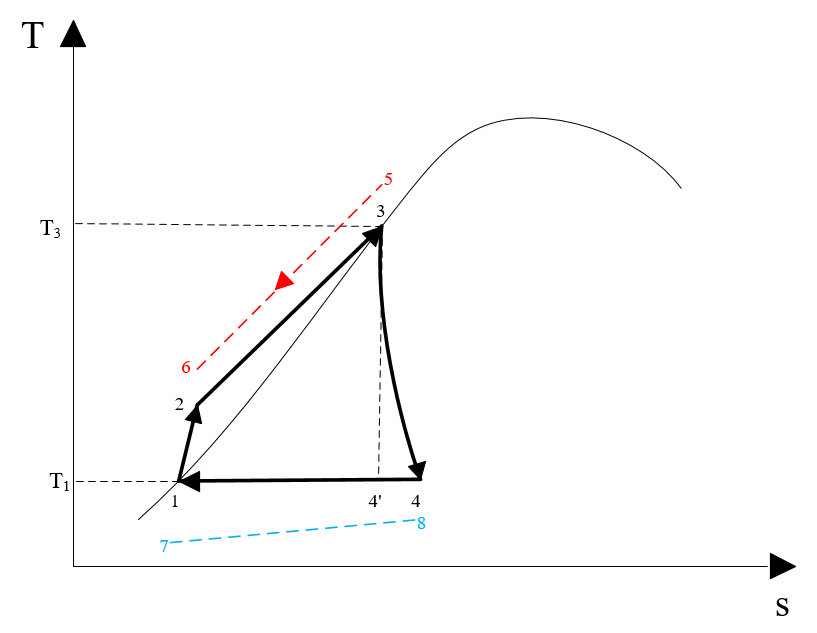
\includegraphics[height=4cm]{images/tfctsdiagram.png}
    \caption{\scriptsize Temperature (T) versus specific entropy (s) diagram of TFC \cite{smith2014power}}
    \label{fig:tlctsdiagram}
    \end{figure}
\end{columns}
\end{frame}

\begin{frame}{Trilateral Flash Closed Cycle (TFC) in NOHTFPECGPPIE}
\begin{columns}
    \column{0.45\textwidth}
    \begin{figure}[h]
      \centering
      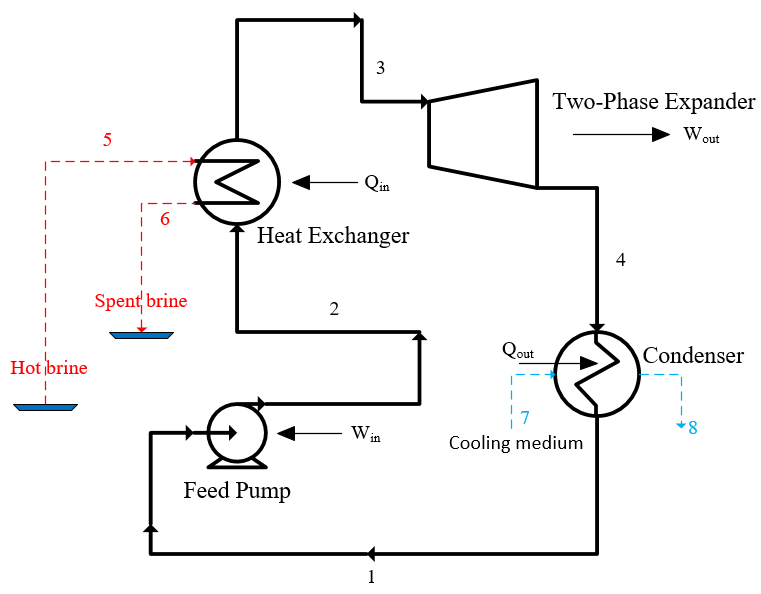
\includegraphics[height=4cm]{images/TLC.png}
      \caption{\scriptsize Schematic Diagram of an Actual Trilateral Closed Cycle (TFC) \cite{smith2014power}}
   \end{figure}
   \column{0.45\textwidth}
    \begin{figure}[h]
    \centering
    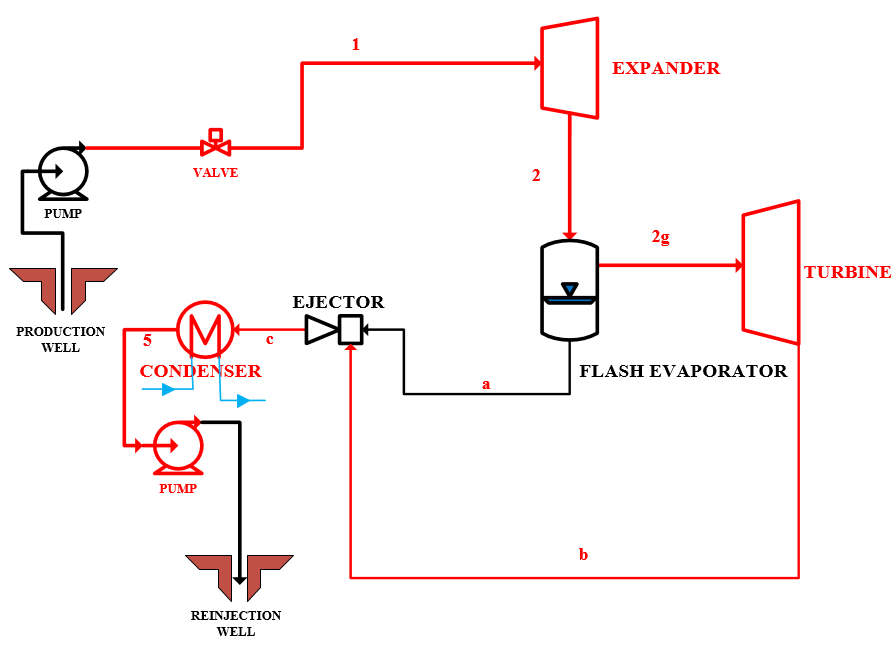
\includegraphics[height=4cm]{images/nohtfpecgppietfc1.png}
    \caption{\scriptsize NOHTFPECGPPIE emphasizing the TFC}
    \end{figure}
\end{columns}
\end{frame}

\begin{frame}{TFC versus BORC}
\begin{columns}
    \column{0.45\textwidth}
    \begin{figure}[h]
      \centering
      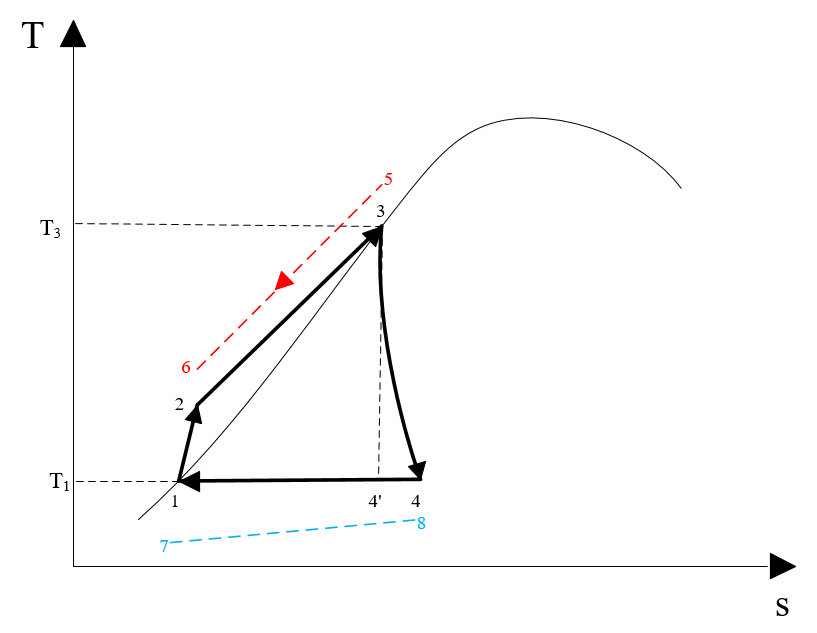
\includegraphics[height=4cm]{images/tfctsdiagram.png}
      \caption{\scriptsize \centering Temperature (T) versus specific entropy (s) diagram of TFC \cite{smith2014power}}
   \end{figure}
   \column{0.45\textwidth}
    \begin{figure}[h]
    \centering
    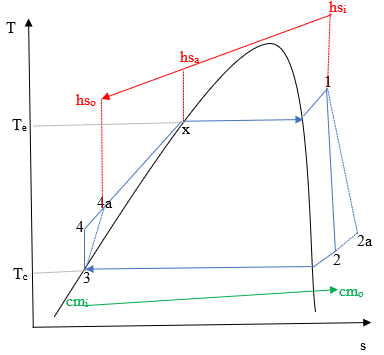
\includegraphics[height=4cm]{images/borctsdiagram.png}
    \caption{\scriptsize \centering Temperature (T) versus specific entropy (s) diagram of Basic Organic Rankine Cycle (BORC)}
    \end{figure}
\end{columns}
\end{frame}

\begin{frame}{TFC versus NOHTFPECGGIE}
\begin{columns}
    \column{0.45\textwidth}
    \begin{figure}[h]
      \centering
      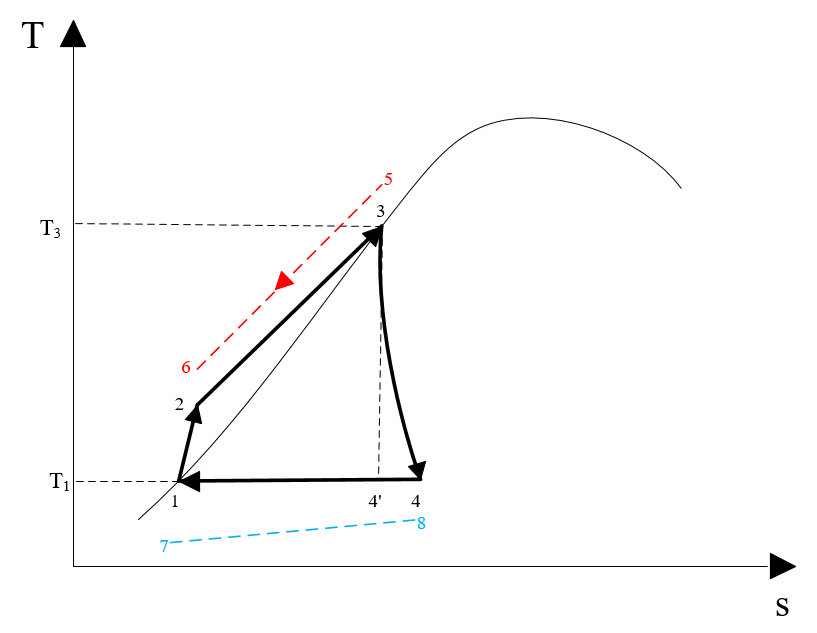
\includegraphics[height=4cm]{images/tfctsdiagram.png}
      \caption{\scriptsize \centering Temperature (T) versus specific entropy (s) diagram of TFC \cite{smith2014power}}
   \end{figure}
   \column{0.45\textwidth}
    \begin{figure}[h]
    \centering
    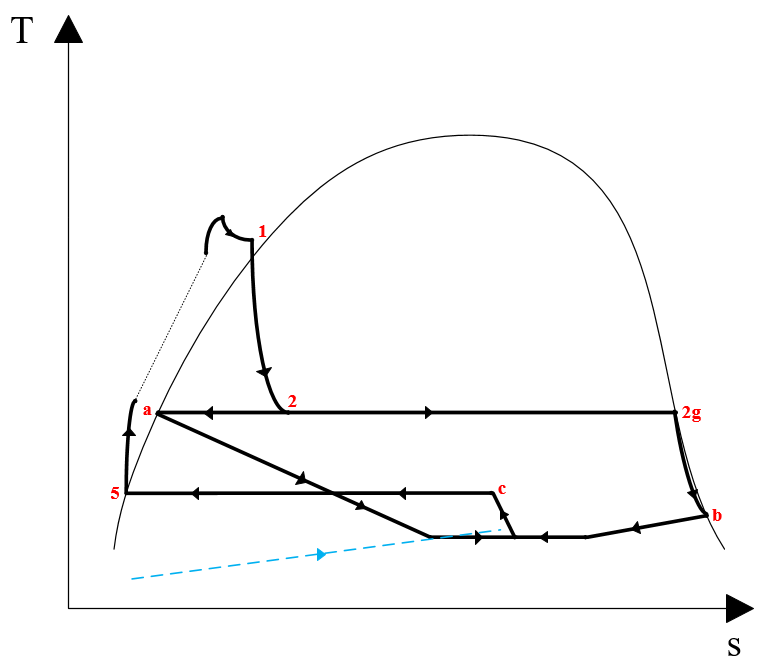
\includegraphics[height=4cm]{images/nohtfpecgppietsdiagram1.png}
    \caption{\scriptsize \centering Temperature (T) versus specific entropy (s) diagram of NOHTFPECGPPIE}
    \end{figure}
\end{columns}
\end{frame}

\begin{frame}{Trilateral Flash Closed Cycle (TFC) Literature}
    \begin{block}{Fischer et al. 2011 \cite{fischer2011comparison}}
    \begin{itemize}
        \item Pros: \textbf{Exergy Efficiency for power production} is \textbf{larger by 14\%-29\%} for the \textbf{Optimized TFC than for the Optimized Organic Rankine Cycle (BORC)} five pairs of temperature ranges.
        \item Cons: TFC has \textbf{Large Volume Expansion Ratios at the Expander} that ranges from \textbf{700-5500} given five pairs of temperature ranges.
        \item Analysis: Thermodynamic Comparative Analysis between TFC and BORC.
        \item  Working Fluid: Water for TFC and Pure Organic Fluid for BORC
        \item Temperature Range: Five pair cases of Evaporating and Condensing Temperatures: (350$^\circ$C,62$^\circ$C), (280$^\circ$C,62$^\circ$C), (280$^\circ$C,15$^\circ$C), (220$^\circ$C,15$^\circ$C) and (150$^\circ$C,15$^\circ$C).
    \end{itemize}
    \end{block}
\end{frame}

\begin{frame}{Trilateral Flash Closed Cycle Literature}
    \begin{block}{Ajimotokan et al. 2014\cite{ajimotokan2014trilateral}}
     \begin{itemize}
         \item Findings: \textbf{30\% to 40\% improvement of thermal efficiency over Organic Rankine} having an Exergy Efficiency of 81.1\%.
         \item Analysis: Thermodynamic Analysis
         \item Working Fluid: Isobutane
         \item Temperature Range: 363-393 K
     \end{itemize}
    \end{block}
\end{frame}

\begin{frame}{Trilateral Flash Closed Cycle Literature}
    \begin{block}{Ajimotokan and Sher (2015)\cite{ajimotokan2015thermodynamic}}
    \begin{itemize}
        \item Findings:
     \begin{table}[h]
         \centering
         \begin{tabular}{cc}
         \hline
             Types of Trilateral Cycles & Thermal Efficiency Range \\
        \hline
              Simple & 11.85-21.97\% \\
              Recuperated & 12.32-23.91\% \\
              Reheat & 11.86-22.07\% \\
              Regenerative & 12.01-22.9\% \\
        \hline
         \end{tabular}
     \end{table}
         \item Working Fluid: N-pentane
         \item Analysis: Thermodynamic Analysis
         \item Temperature Range: 393-443 K
     \end{itemize}
    \end{block}
\end{frame}

\begin{frame}{Trilateral Flash Closed Cycle Literature}
    \begin{block}{Bianchi et al. 2017\cite{bianchi2017numerical}}
     \begin{itemize}
         \item Remarks: Development of a Plug and Play or Packaged type Trilateral Flash Cycle system
         \item Findings: Expected recovered power is 120 kWe and a thermal efficiency of 6\%.
         \item Working Fluid: R1233zd(E) and R245fa
         \item Analysis: Thermodynamic Analysis
     \end{itemize}
    \end{block}
\end{frame}

\begin{frame}{Trilateral Flash Closed Cycle Literature}
    \begin{block}{Li et al. 2017\cite{li2017comparison}}
     \begin{itemize}
         \item Pros: Trilateral Flash Cycle obtains a \textbf{maximum thermal efficiency} of \textbf{14.8\%} at an evaporation temperature of 153$^\circ$C, which is \textbf{40\% higher than that Organic Rankine Cycle} (10.6\%) and \textbf{57\% higher than that of Organic Flash Cycle}. Thermal efficiency of TFC becomes larger than BORC when the evaporation temperature exceeds by 130$^\circ$C.
         \item Cons: It has the \textbf{largest UA value} ranging from \textbf{7.9 kW/$^\circ$C to 8.8 kW/$^\circ$C} for \textbf{evaporation temperatures} of \textbf{100$^\circ$C} to \textbf{150$^\circ$C}, respectively.
         \item Analysis: Thermodynamic Analysis
         \item Working Fluid: R245fa
     \end{itemize}
    \end{block}
\end{frame}

\begin{frame}{Trilateral Flash Closed Cycle Literature}
    \begin{block}{Li et al. 2019\cite{li2019analysis}}
     \begin{itemize}
         \item Remarks: Toluene has the best performance at high-temperature evaporator of 530 K and low-temperature evaporator of 373 K having a maximum power output of 11.3 kW, thermal efficiency of 24.2\% and exergy efficiency of 63.2\%.
         \item Cycle: Combined TLC-ORC
         \item Analysis: Thermodynamic Analysis
         \item Working Fluid for ORC (High Temperature Cycle): Choice of Cyclohexane, Toluene, Benzene and Water
         \item Working Fluid for TLC (Low Temperature Cycle): R245fa
     \end{itemize}
    \end{block}
\end{frame}

\begin{frame}{Trilateral Flash Closed Cycle Literature}
    \begin{block}{Iqbal et al. 2019 \cite{iqbal2019trilateral}}
     \begin{itemize}
         \item Remarks: 
         \begin{enumerate}
             \item TFC has the capability of about \textbf{140\% more power generation than ORC} for the same heat source and sink temperatures.
             \item TFC can be utilized up to \textbf{70\% of available thermal energy} where ORC can only deal with 20\%.
             \item TFC \textbf{allows the heat carrier to leave the system very close to ambient temperature that contribute almost zero to global warming}.
             \item TFC incorporate \textbf{high pumping power} and \textbf{larger heat exchanger and condenser which increases the cost of construction} though it can be compensated by high power generation.
         \end{enumerate}
         \item Analysis: Thermodynamic Analysis, Working Fluid: R1233zd(E)
         \item Heat Source Temperature: 80$^\circ$C, Heat Sink Temperature: Ambient Temperature
     \end{itemize}
    \end{block}
\end{frame}

\begin{frame}{Partial Evaporation Cycles}
\begin{columns}
    \column{0.45\textwidth}
    \begin{figure}[h]
      \centering
      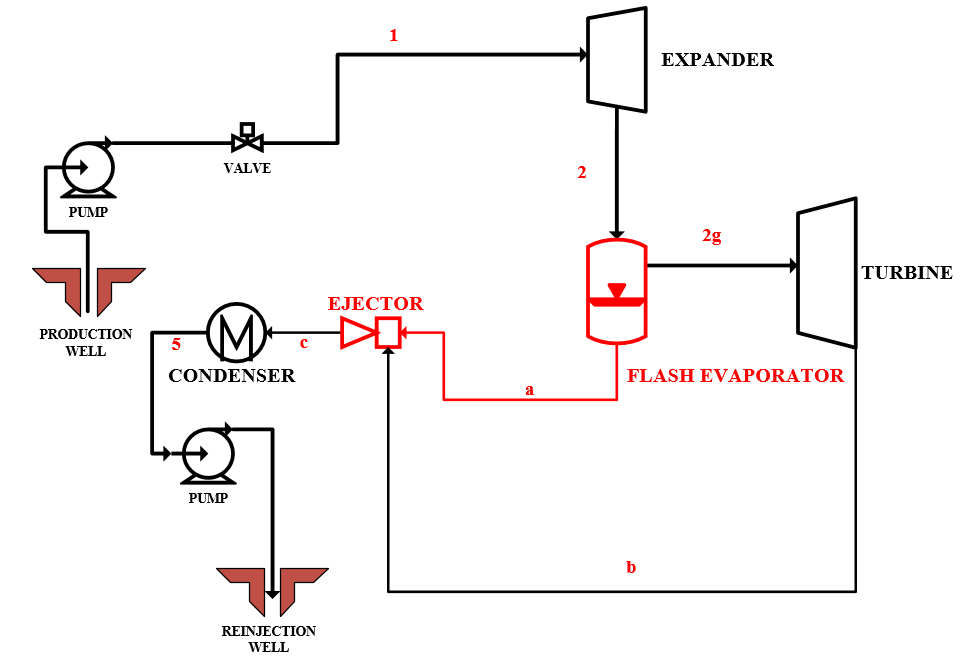
\includegraphics[height=4cm]{images/nohtfpecgppiepe.png}
      \caption{\scriptsize Schematic Diagram of NOHTFPECGPPIE emphasizing the Partial Evaporation}
   \end{figure}
   \column{0.45\textwidth}
    \begin{figure}[h]
    \centering
    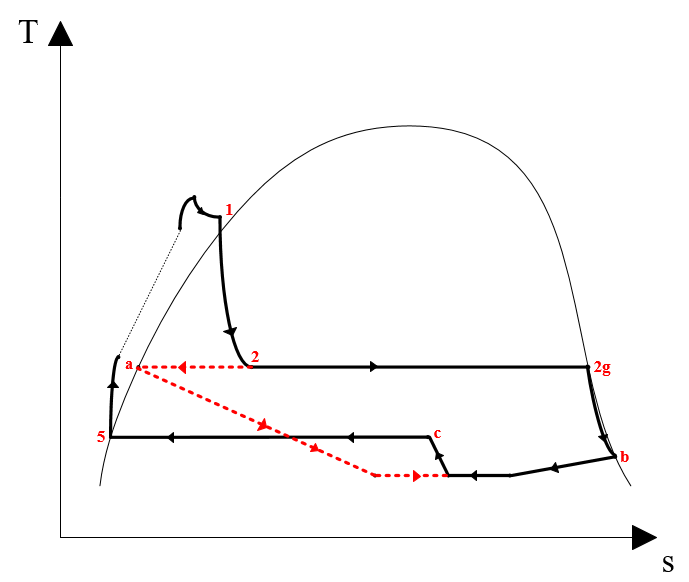
\includegraphics[height=4cm]{images/nohtfpecgppietsdiagram2.png}
    \caption{\scriptsize Temperature (T) versus specific entropy (s) of the NOHTFPECGPPIE}
    \end{figure}
\end{columns}
\end{frame}

\begin{frame}{Effect of the Quality (X) of the Motive Fluid (i.e. at state point a) to the Entrainment Ratio ($\mu$)\cite{wang2016experimental}}
\begin{columns}
    \column{0.45\textwidth}
    \begin{figure}[h]
      \centering
      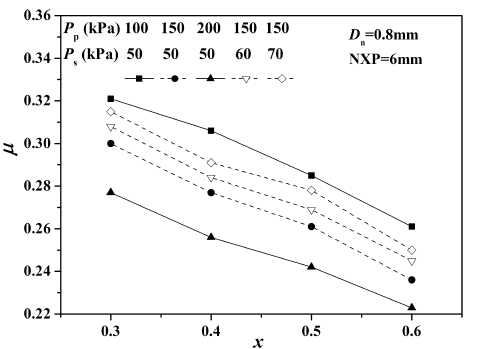
\includegraphics[height=4cm]{images/partialevapmu.png}
      \caption{\scriptsize \centering Effect of the quality (x) to the entrainment ratio ($\mu$) by Wang and Yu (2016) \cite{wang2016experimental}}
   \end{figure}
   \column{0.45\textwidth}
    \begin{block}{Reference}
     Experimental Investigation on two-phase driven ejector performance in a novel ejector enhanced refrigeration system by Wang and Yu 2016 \cite{wang2016experimental}
    \end{block}
    \begin{block}{Entrainment Ratio ($\mu$), Quality (x)}
     $\mu = \frac{\Dot m_{s}}{\Dot m_{p}}$, \: $x = \frac{Volume\:of\:the\:vapor}{Total\:volume\:of \:the\:mixture}$
    \end{block}
\end{columns}
\end{frame}

\begin{frame}{Effect of the Quality (X) of the Motive Fluid (i.e. at state point a) to the Pressure Ratio ($r_{p}$)\cite{wang2016experimental}}
\begin{columns}
    \column{0.45\textwidth}
    \begin{figure}[h]
      \centering
      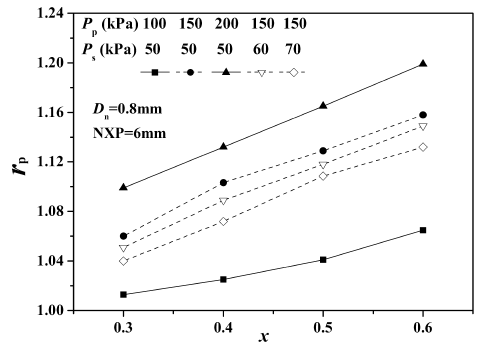
\includegraphics[height=4cm]{images/partialevaprp.png}
      \caption{\scriptsize \centering Effect of the quality (x) to the pressure ratio ($r_{p}$) by Wang and Yu (2016) \cite{wang2016experimental}}
   \end{figure}
   \column{0.45\textwidth}
    \begin{block}{Reference}
     Experimental Investigation on two-phase driven ejector performance in a novel ejector enhanced refrigeration system by Wang and Yu 2016 \cite{wang2016experimental}
    \end{block}
    \begin{block}{Pressure Ratio ($r_{p}$), Quality (x)}
     $r_{p} = \frac{P_{d}}{P_{s}}$, \: $x = \frac{Volume\:of\:the\:vapor}{Total\:volume\:of \:the\:mixture}$
    \end{block}
\end{columns}
\end{frame}

\begin{frame}{Effect of the Quality (X) of the Motive Fluid (i.e. at state point a) to the Ejector Efficiency ($\eta$) \cite{wang2016experimental}}
\begin{columns}
    \column{0.45\textwidth}
    \begin{figure}[h]
      \centering
      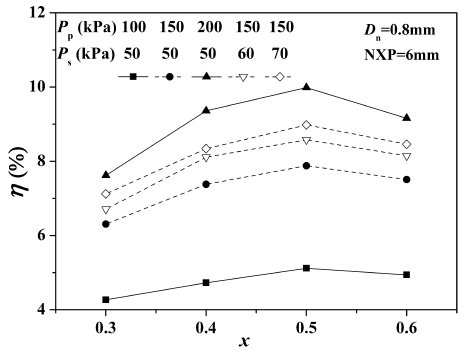
\includegraphics[height=4cm]{images/partialevapejeceff.png}
      \caption{\scriptsize \centering Effect of the quality (x) to the ejector efficiency ($\eta$) by Wang and Yu (2016) \cite{wang2016experimental}}
   \end{figure}
   \column{0.45\textwidth}
    \begin{block}{Ejector Efficiency ($\eta$)}
    Ratio of the actual expansion work recovered by the the ejector $(\Dot W_{rec})$ to the maximum possible work rate recovery $(\Dot W_{rec,max})$
        \begin{equation}
            \eta = \frac{\Dot W_{rec}}{\Dot W_{rec,max}} = \frac{\Dot m_{s}(h_{d}-h_{s})}{\Dot m_{p}(h_{p}-h_{d})}
        \end{equation}
    \end{block}
\end{columns}
\end{frame}

\begin{frame}{Ejector}
\begin{columns}
  \column{0.45\textwidth}
  \begin{block}{Ejector}
   Tashtoush et al.\cite{tashtoush2019comprehensive} defines Ejector as a flow device with two intake ports and one discharge that allows the primary high-pressure stream to entrain the secondary low-pressure stream, where both streams are being mixed inside the ejector and discharged at some intermediate pressure termed as backpressure.
  \end{block}
  \column{0.45\textwidth}
  \begin{figure}[h]
   \centering
   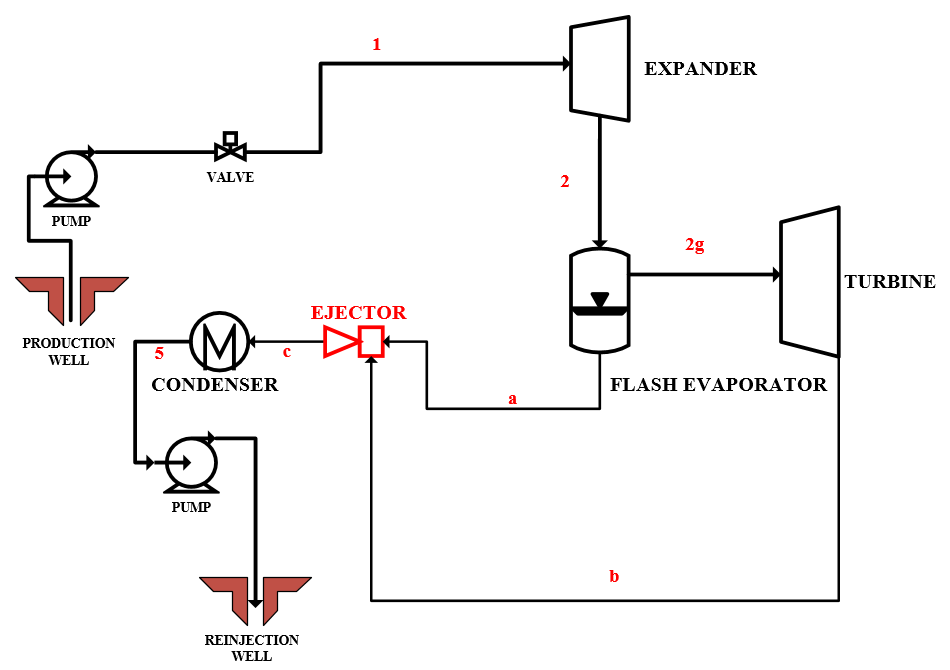
\includegraphics[height=4cm]{images/nohtfpecgppieejector.png}
   \caption{Emphasizing Ejector in NOHTFPECGPPIE}
  \end{figure}
  \end{columns}
\end{frame}

\begin{frame}{Basic Parts of an Ejector drawn using ANSYS R18.0}
  \begin{figure}[h]
    \centering
   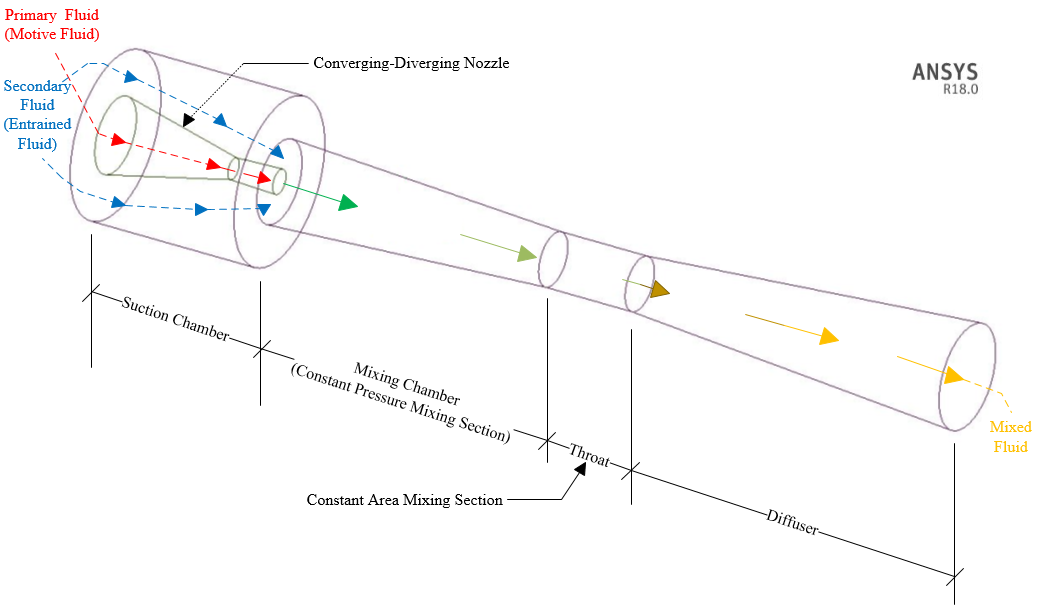
\includegraphics[height=5.25cm]{images/Ejector basic parts.PNG}
    \label{fig:ejectorparts}
  \end{figure}  
\end{frame}

\begin{frame}{Rationale of the Construction of the Ejector}
    \begin{block}{Tashtoush et al. \cite{tashtoush2019comprehensive}}
     Moving the converging-diverging nozzle discharge port away from the ejector's throat (upstream the entrance) would enhance the performance of the ejector by augmenting the entrainment ratio.
    \end{block}
    \begin{block}{Definition of Entrainment Ratio}
     Entrainment Ratio is defined as the ratio of the secondary mass flow rate to the primary mass flow rate. 
    \end{block}
\end{frame}

\begin{frame}{Rationale of the Construction of the Ejector}
    \begin{block}{Pianthong et al.\cite{pianthong2007investigation}}
     The enhancement of the entrainment ratio is occurred when the nozzle exit was positioned away from the ejector throat.\textbf{Positioning the nozzle exit away from the ejector throat increases the effective area of the hypothetical throat between the jet core (steam jet) and ejector wall (mixing nozzle) at which the secondary was entrained before mixing occurred.}
    \end{block}
    \begin{figure}
        \centering
        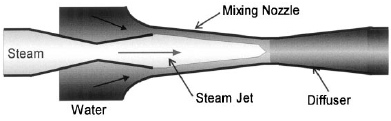
\includegraphics[height=2cm]{images/Central steam jet.PNG}
        \caption{\small Central Steam Jet Ejector based on the illustration of Narabayashi et al. \cite{narabayashi1997study,narabayashi2000study}}
        \label{fig:centralsteamjet}
    \end{figure}
\end{frame}

\begin{frame}{Rationale of the Construction of the Ejector}
    \begin{block}{Chunnanond and Aphornratana\cite{chunnanond2004experimental}}
     When the NXP is moved away from the ejector throat, the expansion waves of the jet core stream would face stronger compression effect and, consequently, smaller expansion angle and larger effective area would be produced.
    \end{block}
\end{frame}

\begin{frame}{Ejectors: Operating Principles}
    \begin{columns}
    \column{0.45\textwidth}
    \begin{figure}[h]
      \centering
      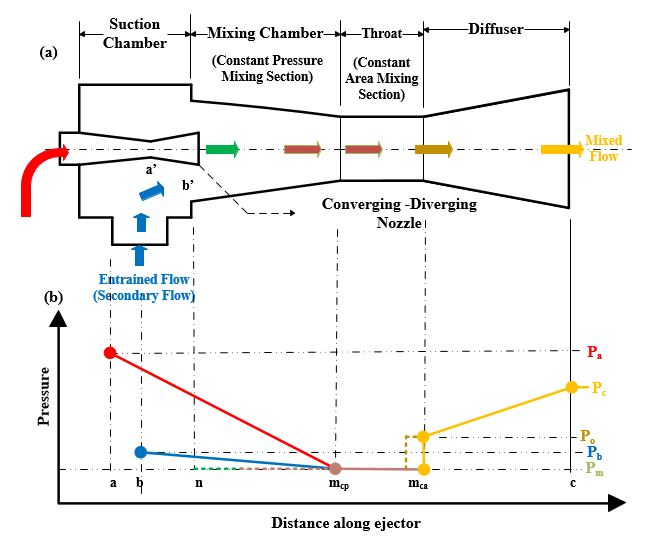
\includegraphics[height=4cm]{images/Ejectorpressureprofile1.JPG}
      \caption{\scriptsize Pressure Profile versus distance along ejector}
   \end{figure}
   \column{0.45\textwidth}
    \begin{figure}[h]
    \centering
    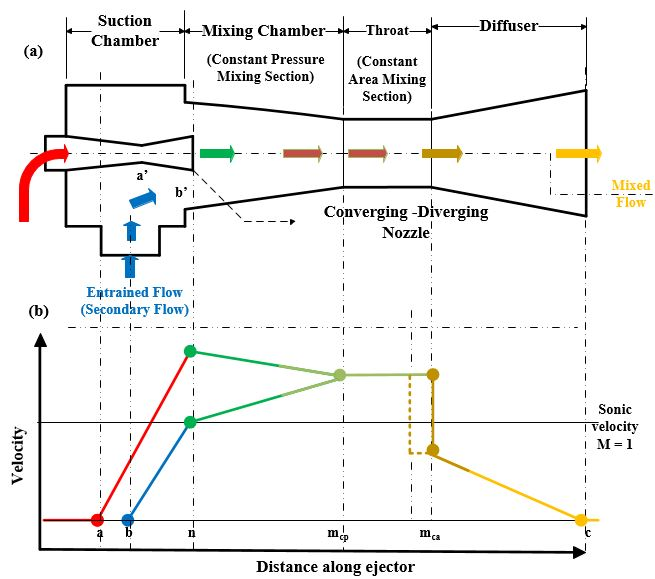
\includegraphics[height=4cm]{images/EjectorVelocityprofile.JPG}
    \caption{\scriptsize Velocity Profile versus distance along ejector}
    \end{figure}
\end{columns}
\end{frame}

\begin{frame}{Ejectors: Operating State Conditions}
    \begin{figure}[h]
    \centering
   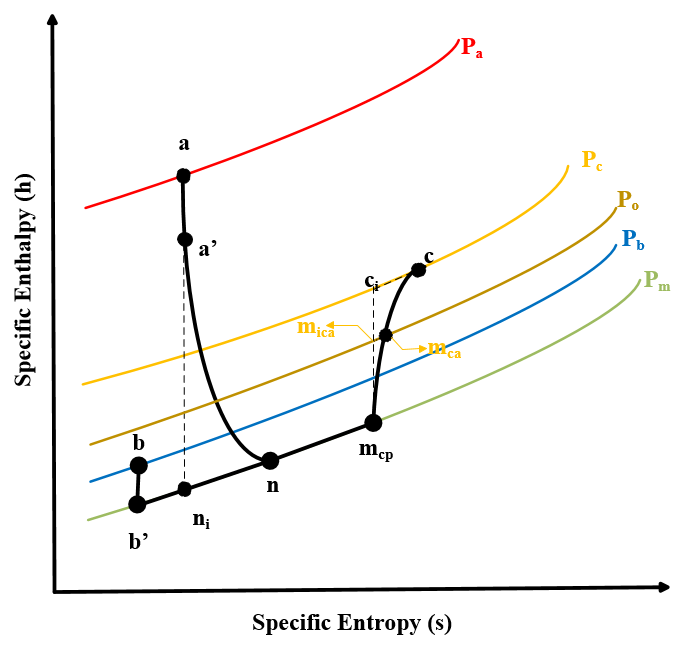
\includegraphics[height=4.5cm]{images/ejectorhsd.PNG}
    \caption{\scriptsize \centering Specific enthalpy (h) – Specific entropy (s) diagram of the processes inside the single-phase subsonic ejector}
    \label{fig:ejectorhsd}
\end{figure}
\end{frame}

\begin{frame}{Different types of ejector based on the location of the converging-diverging nozzle\cite{huang1985ejector}}
  \begin{columns}
    \column{0.45\textwidth}
    \begin{figure}[h]
      \centering
      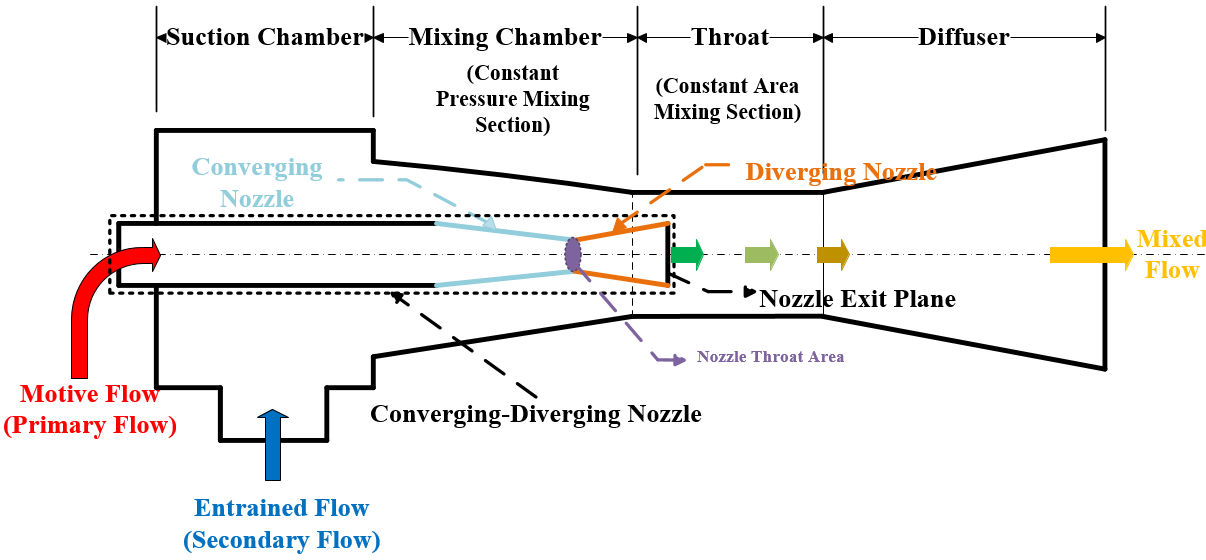
\includegraphics[height=2.5cm]{images/CAM ejector.PNG}
      \caption{CAM Ejector}
   \end{figure}
   \column{0.45\textwidth}
    \begin{figure}[h]
    \centering
    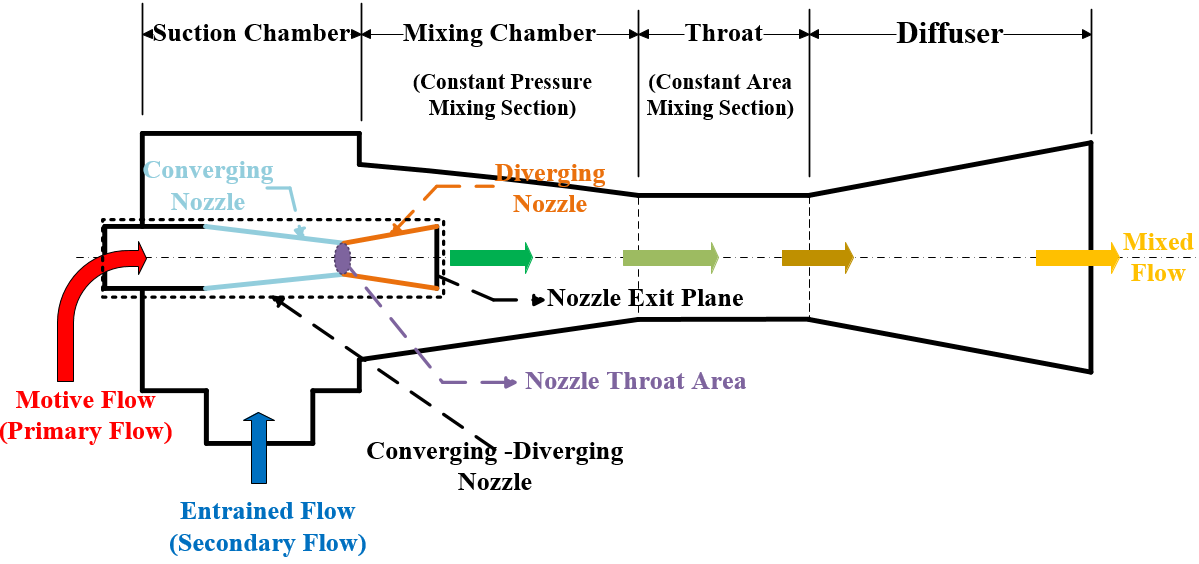
\includegraphics[height=2.5cm]{images/CPM ejector.PNG}
    \caption{CPM Ejector}
    \end{figure}
  \end{columns}
\end{frame}

\begin{frame}{Different Locations of Nozzle Exit Positions (NXP) of Ejector\cite{eames1999experimental,eames2007results,kumar2019effect,wang2017numerical, ramesh2018experimental, meyer2009steam}}
\begin{columns}
    \column{0.45\textwidth}
    \begin{figure}
        \centering
        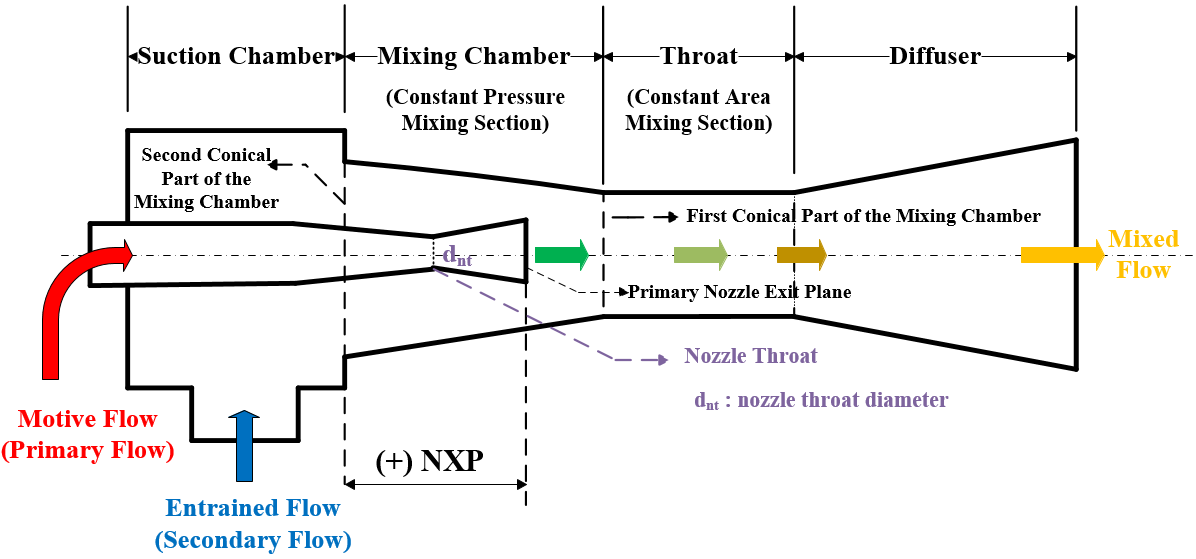
\includegraphics[height=2.5cm]{images/NXP+.PNG}
        \caption{\centering Positive NXP}
        \label{fig:nxppositive}
    \end{figure}
    \column{0.45\textwidth}
    \begin{figure}
        \centering
        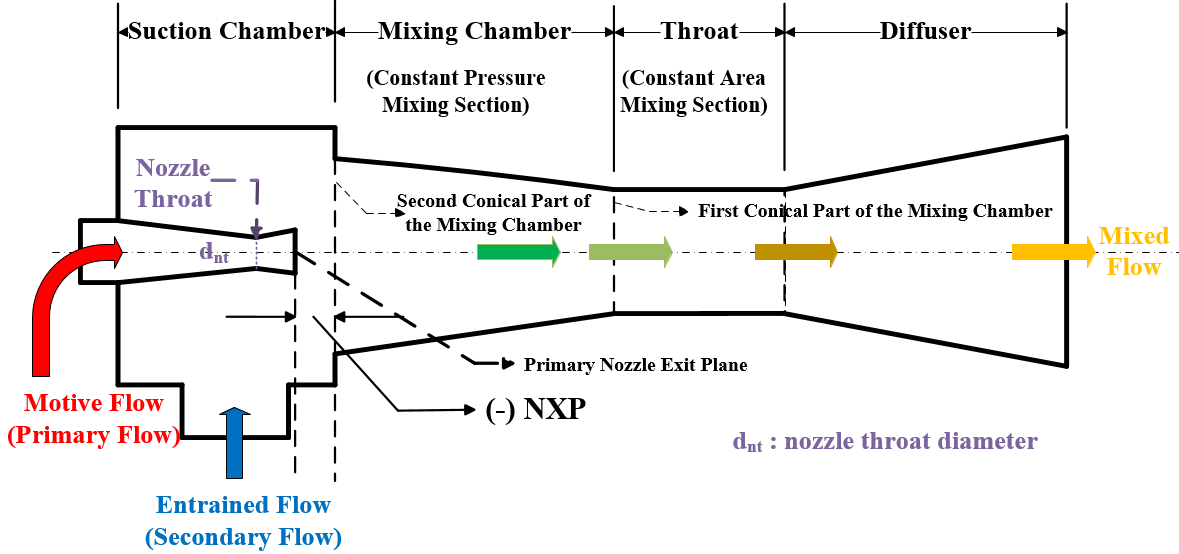
\includegraphics[height=2.5cm]{images/NXP-.PNG}
        \caption{\centering Negative NXP}
        \label{fig:nxpnegative}
    \end{figure}
\end{columns}
\end{frame}

\begin{frame}{Different Locations of Nozzle Exit Position (NXP) of Ejector\cite{eames1999experimental,eames2007results,kumar2019effect,wang2017numerical, ramesh2018experimental, meyer2009steam}}
    \begin{figure}
        \centering
        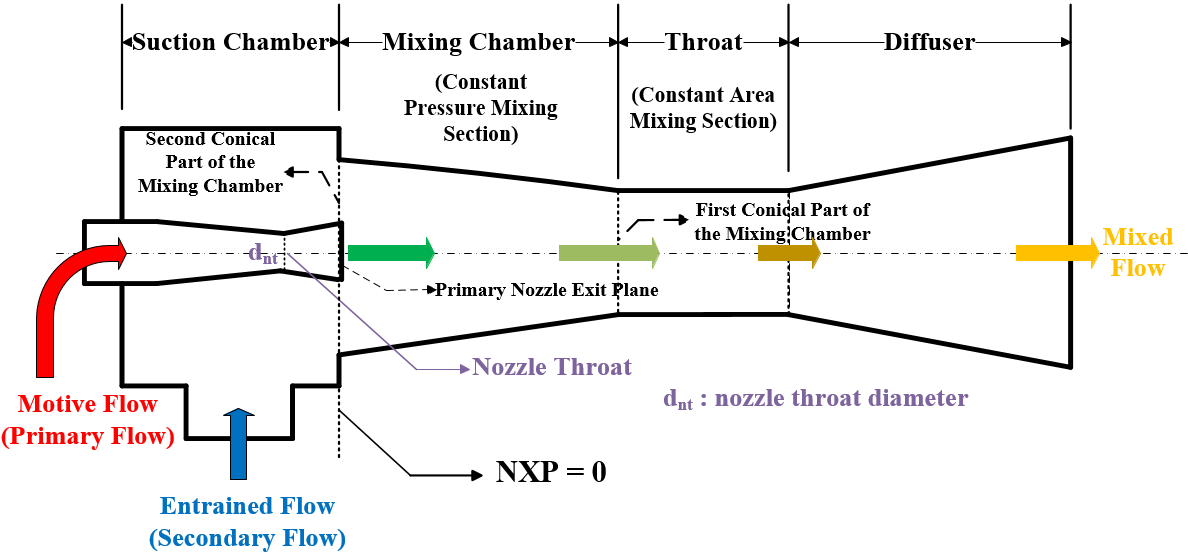
\includegraphics[height=3.5cm]{images/NXP0.PNG}
        \caption{\centering Zero NXP}
        \label{fig:nxpnxpzero}
    \end{figure}
\end{frame}

\begin{frame}{CAM and CPM Ejector: Review of Literature}
    Keenan et al. \cite{keenan1950investigation} proposed the concept of CPM ejector. Although CAM ejector can provide higher mass flow rates, the CPM ejectors are considered to be more favorable in practice for the merit of its stable performance at a wider range of backpressures \cite{tashtoush2019comprehensive}.
\end{frame}

\begin{frame}{Effect of NXP on the performance of the ejector\cite{tashtoush2019comprehensive}}
    \begin{table}[h]
        \centering
        \begin{tabular}{|p{2cm}|p{1.5cm}|p{4.5cm}|}
        \hline
            Model & Working Fluid & NXP\\
        \hline
             Experimental\cite{eames1999experimental} & Steam & Optimum (NXP/throat diameter) were found to vary in the range of -0.5 to 0.5 for a primary pressure ratio of 1.07 to 0.75, respectively \\
        \hline
             CFD and Experimental\cite{wang2018auto} & Methanol & Optimum NXP decreases as the primary flow pressure increases \\
        \hline
        \end{tabular}
    \end{table}
\end{frame}

\begin{frame}{Effect of NXP on the performance of the ejector\cite{tashtoush2019comprehensive}}
    \begin{table}[h]
        \centering
        \begin{tabular}{|p{2cm}|p{1.5cm}|p{5cm}|}
        \hline
            Model & Working Fluid & NXP\\
        \hline
             CFD and Experimental\cite{eames2007results} & R245fa & Optimum NXP is 5 mm upstream the entrance given entrainment ratio of 0.567, generator and evaporator temperatures of 120 and 12 $^{\circ}C$\\
        \hline
             Experimental\cite{meyer2009steam} & Steam & Optimum NXP is 5 mm upstream the entrance at boiler temperature of 85 to 110$^{\circ}C$ \\
        \hline
        \end{tabular}
    \end{table}
\end{frame}

\begin{frame}{Effect of NXP on the performance of the ejector\cite{tashtoush2019comprehensive}}
    \begin{table}[h]
        \centering
        \begin{tabular}{|p{2cm}|p{1.5cm}|p{4.5cm}|}
        \hline
            Model & Working Fluid & NXP\\
        \hline
             CFD \cite{varga2009influence} & Steam & Optimum NXP is 6 mm downstream the entrance\\
        \hline
             CFD\cite{zhu2009numerical} & R141a & Optimum (NXP/Diffuser throat diameter) is in the range of 1.7-3.4 upstream the entrance\\
        \hline
        \end{tabular}
    \end{table}
\end{frame}

\begin{frame}{Effect of NXP on the performance of the ejector\cite{tashtoush2019comprehensive}}
    \begin{table}[h]
        \centering
        \begin{tabular}{|p{2cm}|p{1.5cm}|p{5cm}|}
        \hline
            Model & Working Fluid & NXP\\
        \hline
             CFD \cite{yan2012geometry} & R134a & Optimum NXP is 8.91 mm upstream of the entrance\\
        \hline
             Experimental\cite{yapici2008experimental} & R123 & Among the tested ejectors it was found that optimum NXP values are always within -10 mm to 5 mm at which minimum suction pressure occurs in the suction chamber\\
        \hline
        \end{tabular}
    \end{table}
\end{frame}

\begin{frame}{Effect of NXP on the performance of the ejector\cite{tashtoush2019comprehensive}}
    \begin{table}[h]
        \centering
        \begin{tabular}{|p{2cm}|p{1.5cm}|p{5cm}|}
        \hline
            Model & Working Fluid & NXP\\
        \hline
             Experiment \cite{chunnanond2004ejectors} & Steam & Expansion waves of the jet core stream face stronger compression effect as NXP is moved upstream. Thus, a smaller expansion angle and a larger effective area would be produced\\
        \hline
             CFD\cite{hakkaki2015computational} & --- & Optimum NXP is 13 mm\\
        \hline
        \end{tabular}
    \end{table}
\end{frame}

\begin{frame}{Effect of NXP on the performance of the ejector\cite{tashtoush2019comprehensive}}
    \begin{table}[h]
        \centering
        \begin{tabular}{|p{2cm}|p{1.5cm}|p{5.5cm}|}
        \hline
            Model & Working Fluid & NXP\\
        \hline
             CFD \cite{omidvar2016entropy} & --- & Optimum NXP is 5 mm upstream corresponding to an improvement in performance of 37\% relative to the original geometry before optimization  \\
        \hline
             CFD\cite{chen2013numerical} & Natural gas & Maximum entrainment ratio is attained when the NXP is in the range of 3.6 to 7.2 mm. For optimum pressure ratio, NXP to be in the range of 1.2-7.2 mm\\
        \hline
        \end{tabular}
    \end{table}
\end{frame}

\begin{frame}{Effect of NXP on the performance of the ejector\cite{tashtoush2019comprehensive}}
    \begin{table}[h]
        \centering
        \begin{tabular}{|p{2cm}|p{1.5cm}|p{5cm}|}
        \hline
            Model & Working Fluid & NXP\\
        \hline
             Experiment\cite{jeon2017performance} & R600a for two-phase ejector & Maximum pressure lifting ratio was observed at NXP is 3 mm  \\
        \hline
             Numerical study\cite{pei2019numerical} & Hydrogen & The hydrogen entrainment ratio decreases dramaticallly in the whole operating range when NXP is above the optimal value range\\
        \hline
        \end{tabular}
    \end{table}
\end{frame}

\begin{frame}{Effect of NXP on the performance of the ejector\cite{tashtoush2019comprehensive}}
    \begin{table}[h]
        \centering
        \begin{tabular}{|p{2cm}|p{1.5cm}|p{5cm}|}
        \hline
            Model & Working Fluid & NXP\\
        \hline
             Experiment\cite{jeon2017performance} & R600a for two-phase ejector & Maximum pressure lifting ratio was observed at NXP is 3 mm  \\
        \hline
             Numerical study\cite{pei2019numerical} & Hydrogen & The hydrogen entrainment ratio decreases dramaticallly in the whole operating range when NXP is above the optimal value range\\
        \hline
        \end{tabular}
    \end{table}
\end{frame}

\begin{frame}{Effect of NXP on the performance of the ejector\cite{tashtoush2019comprehensive}}
    \begin{table}[h]
        \centering
        \begin{tabular}{|p{2cm}|p{1.5cm}|p{5cm}|}
        \hline
            Model & Working Fluid & NXP\\
        \hline
             Experiment and Numerical\cite{chong2014experimental} & --- & There exists an optimal NXP corresponding to maximum entrainment ratio, but the critical value of discharged pressure is almost independent of NXP  \\
        \hline
        \end{tabular}
    \end{table}
\end{frame}

\begin{frame}{Applications of Commercially Available Steam Ejector\cite{SchutteandKoerting}}
  \begin{columns}
    \column{0.45\textwidth}
    \begin{itemize}
        \item Supplying heated water to jackets of stills and graining bowls
        \item Intermittent pumping of liquids from tanks and pits
        \item Condensing and mixing ammonia
        \item Pipeline heater
        \item Pumping waste water from quench tanks and cleaning inline pipes with heated water in steel processing
    \end{itemize}
    \column{0.45\textwidth}
    \begin{figure}
        \centering
        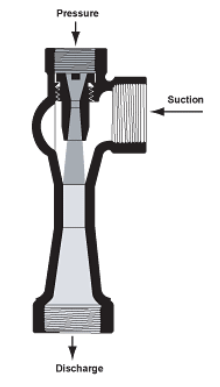
\includegraphics[height=4.5cm]{images/schutteandkoertingthermosyphon.png}
        \caption{\centering Steam Jet Syphon(Commercially Available Steam Ejectors) photo courtesy of Schutte and Koerting \cite{SchutteandKoerting}}
    \end{figure}
  \end{columns}
\end{frame}

\begin{frame}{Applications of Commercially Available Steam Ejector\cite{SchutteandKoerting}}
  \begin{columns}
    \column{0.45\textwidth}
    \begin{itemize}
        \item Used on dust collecting equipment
        \item Used for draining large receptacles of waste process
        \item Condensing and mixing ammonia
        \item Automatic pumping of chemical spill
        \item Automatic pumping of condensate sump for power industry
    \end{itemize}
    \column{0.45\textwidth}
    \begin{figure}
        \centering
        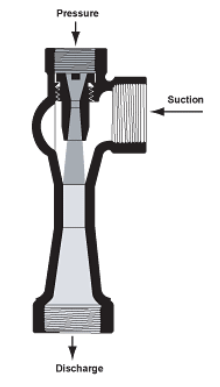
\includegraphics[height=4.5cm]{images/schutteandkoertingthermosyphon.png}
        \caption{\centering Steam Jet Syphon(Commercially Available Steam Ejectors) photo courtesy of Schutte and Koerting \cite{SchutteandKoerting}}
    \end{figure}
  \end{columns}
\end{frame}

\begin{frame}{Applications of Commercially Available Steam Ejector\cite{SchutteandKoerting}}
  \begin{columns}
    \column{0.45\textwidth}
    \begin{itemize}
        \item Automatic pumping of water in hot house in agricultural industry
        \item Pumping filtrate from vacuum vessels and condensate from surface condensers
        \item Supplying heated water to the jackets of stills and graining bowls
        \item Removing liquid from pickling baths.
        \item Extracting chemicals in reaction chambers
    \end{itemize}
    \column{0.45\textwidth}
    \begin{figure}
        \centering
        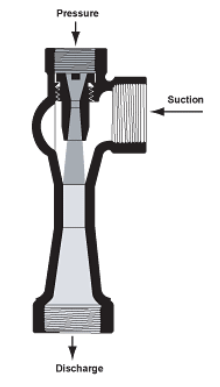
\includegraphics[height=4.5cm]{images/schutteandkoertingthermosyphon.png}
        \caption{\centering Steam Jet Syphon (Commercially Available Steam Ejectors) photo courtesy of Schutte and Koerting \cite{SchutteandKoerting}}
    \end{figure}
  \end{columns}
\end{frame}

\begin{frame}{Applications of Commercially Available Steam Ejector\cite{SchutteandKoerting}}
  \begin{columns}
    \column{0.45\textwidth}
    \begin{itemize}
        \item Moving powdered material or material in granular form
        \item Filling and emptying gas holder tanks
        \item Handling soap solutions in textile plants
        \item Pumping sugar juice and various liquids in canning plants
    \end{itemize}
    \column{0.45\textwidth}
    \begin{figure}
        \centering
        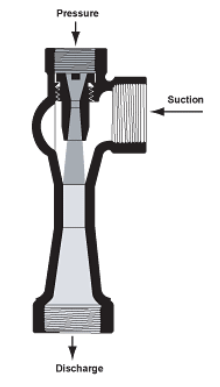
\includegraphics[height=4.5cm]{images/schutteandkoertingthermosyphon.png}
        \caption{\centering Steam Jet Syphon (Commercially Available Steam Ejectors) photo courtesy of Schutte and Koerting \cite{SchutteandKoerting}}
    \end{figure}
  \end{columns}
\end{frame}

\begin{frame}{Commercially Available Steam Ejectors: Steam Jet Syphons\cite{SchutteandKoerting}}
    \begin{table}[h]
    \centering
    \caption{\centering \scriptsize Different Sizes of Steam Jet Syphons based from the Ejector Manufacturer Schutte \& Koerting\cite{SchutteandKoerting}}
    \label{tab:SteamJetSyphons_workingpress}
    \begin{tabular}{|c|c|c|c|c|c|c|}
    \hline
        Size & \multicolumn{3}{c|}{Steam Inlet Pressure (kPa)} & \multicolumn{3}{c|}{Liquid Inlet Pressure (kPa)}\\
    \cline{2-7}
        No. & Cast Iron & Bronze & Stainless Steel & Cast Iron & Bronze & Stainless Steel \\
    \hline
        1 & 1207 & 862 & 3450 & 862 & 690 & 2070 \\
    \hline
        2 & 1207 & 862 & 3450 & 862 & 690 & 2070 \\
    \hline
        3 & 1207 & 862 & 3450 & 862 & 690 & 2070 \\
    \hline
        4 & 1035 & 862 & 3450 & 690 & 690 & 2070 \\
    \hline
        5 & 1035 & 862 & 3450 & 690 & 690 & 2070 \\
    \hline
        6 & 1380 & 1380 & 3450 & 690 & 690 & 2070 \\
    \hline
        \textbf{7} & 1380 & 1380 & \textbf{3450} & 690 & 690 & \textbf{2070} \\
    \hline
        8\textsuperscript{a} & 862 & --- & --- & 862 & --- & --- \\
    \hline
        9\textsuperscript{a} & 862 & --- & --- & 862 & --- & --- \\
    \hline
    \end{tabular}
\end{table}
\end{frame}

\begin{frame}{Dimensions of Different Sizes of Steam Jet Syphons based from the Ejector Manufacturer Schutte \& Koerting\cite{SchutteandKoerting}}
\begin{columns}
    \column{0.45\textwidth}
       \begin{table}[h]
       \label{tab:SteamJetSyphons_sizes}
       \begin{tabular}{|c|c|c|c|}
        \hline
        Size & \multicolumn{3}{c|}{Dimensions (mm)}  \\
        \cline{2-4}
        No & A & B & C \\
        \hline
        1 & 27 & 65 & 29 \\
        \hline
        2 & 35 & 86 & 32 \\
        \hline
        3 & 38 & 110 & 41 \\
        \hline
        4 & 51 & 165 & 51 \\
       \hline
        5 & 57 & 194 & 57 \\
       \hline
        6 & 68 & 235 & 79 \\
       \hline
        \textbf{7} & \textbf{80} & \textbf{286} & \textbf{89} \\
        \hline
        8 & 112 & 490 & 198 \\
        \hline
        9 & 155 & 721 & 232 \\
        \hline
        \end{tabular}
       \end{table}
   \column{0.35\textwidth}
    \begin{figure}[h]
    \centering
    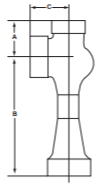
\includegraphics[height=5cm]{images/Syphonsshcutteandkoerting.PNG}
    \end{figure}
  \end{columns}
\end{frame}

\begin{frame}{Steam Jet Vacuum Systems\cite{NASH:Technology}}
    \begin{columns}
    \column{0.45\textwidth}
       \begin{itemize}
           \item \small Uses High-Pressure High-Temperature steam as a motive fluid to entrain the pressurized water in the steam ejector
           \item \small High-pressure high-temperature steam inflowing to the converging-diverging nozzle flushes the non-condensible gases inside the ejector, thus, making it a vacuum system.
           \item \small Steam jet vacuum system is used in large-scale thermal power plants (i.e. large power capacity geothermal power plants), thus making it beyond the scope of this study.
       \end{itemize}
   \column{0.45\textwidth}
    \begin{figure}[h]
    \centering
    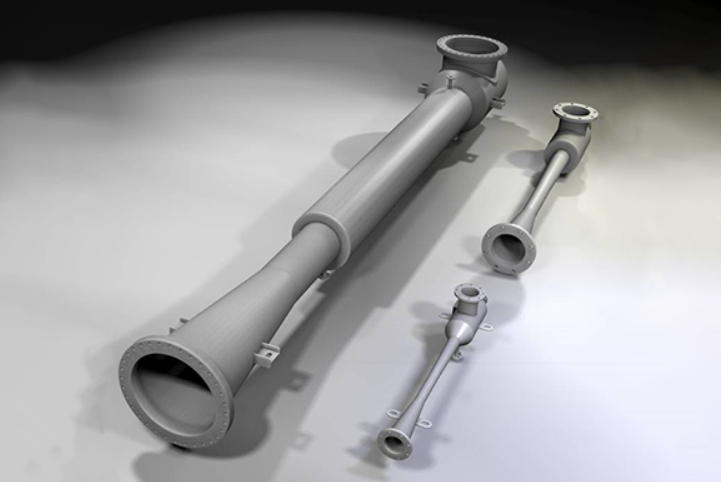
\includegraphics[height=4cm]{images/SteamVacuumsystem.PNG}
    \caption{Photo courtesy of Gardner Denver\cite{NASH:Technology}}
    \end{figure}
  \end{columns}
\end{frame}

\begin{frame}{\small Novel Open Hybrid Trilateral Flash Partial Evaporating Cycle Geothermal Power Plant Incorporated in an Ejector(NOHTFPECGPPIE)}
    \begin{columns}
    \column{0.45\textwidth}
    \begin{figure}[h]
      \centering
      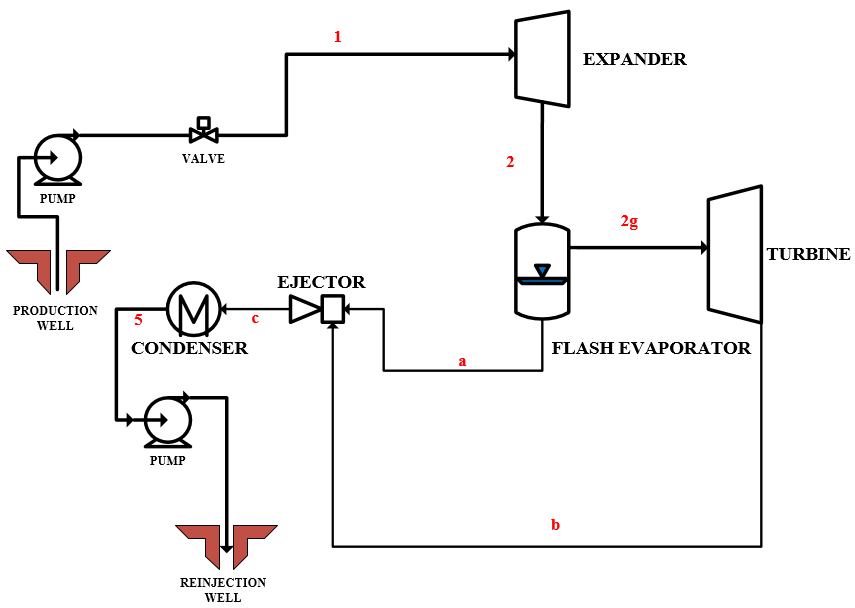
\includegraphics[height=3.5cm]{images/NOHTFPECGPPIE.PNG}
      \caption{\scriptsize \centering Schematic Diagram of the NOHTFPECGPPIE}
      \label{fig:nohtfpecgppieschematicdiagram}
   \end{figure}
   \column{0.45\textwidth}
    \begin{figure}[h]
    \centering
    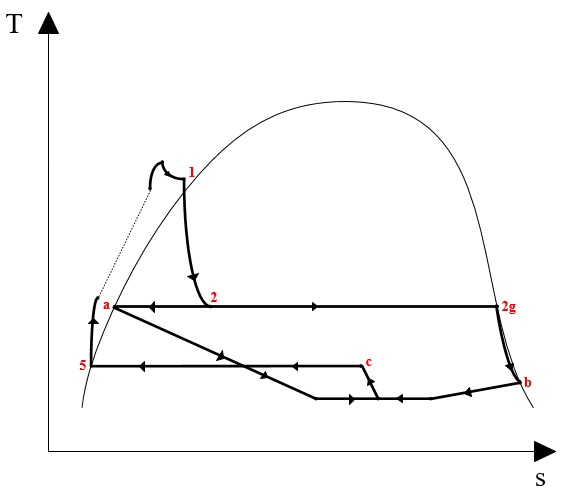
\includegraphics[height=3.75cm]{images/nohtfpecgppietsdiagram.jpg}
    \caption{\scriptsize \centering Temperature (T) versus specific entropy (s) diagram of NOHTFPECGPPIE}
    \label{fig:nohtfpecgppietsdiagram}
    \end{figure}
\end{columns}
\end{frame}

\begin{frame}{Problem Statement}
  \begin{block}{Ideal Situation}
   NOHTFPECGPPIE operates on a driven central water jet steam ejector low-enthalpy-to-power conversion cycle.
  \end{block}
  \begin{block}{Actual Situation}
   \begin{itemize}
       \item Majority of the ejector (especially steam ejector) applies to refrigeration system and less in the power generation systems.
       \item  Majority of the steam ejector in operates on single phase flows and less in two-phase flows.
       \item Two-phase flow steam ejector is flowing at supersonic state uses steam as a motive fluid enough to entrain the liquid water
   \end{itemize}
  \end{block}
\end{frame}

\begin{frame}{Problem Objectives}
    In able to prepare the proposed NOHTFPECGPPIE to execute on a test scale, the following objective must be attained:
   \begin{itemize}
    \item Validate the CFD model of the replicated subsonic steam central core driven ejector design (e.g. SJP3) from the existing experimental data and ejector design of Shah et al. \cite{shah2014experimental} thru ANSYS Fluent R18 software.
    \item After validation, reverse the flow in the steam ejector by using pressurized water as a motive fluid and steam as an entrained fluid and simulate the CFD model using ANSYS Fluent R18 software.
  \end{itemize}
\end{frame}

\begin{frame}{Problem Objectives}
    \begin{itemize}
        \item Investigate the use of a brine as a working fluid replacing of pure water in the steam ejector.The brine properties and geothermal well head pressure are obtained from the slimhole of Tingloy Geothermal Power Plant from the Department of Energy.
        \item Conduct sensitivity analysis in the ejector by conducting a partial evaporation on the pressurized water in the ejector with respect to the given ejector geometries and operating conditions.
       \item Compare the NOHTFPECGPPIE to other power generation cycles that uses low-grade thermal or low-enthalpy as a source of heat energy.
    \end{itemize}
\end{frame}

\begin{frame}{Significance of the Problem}
    The study about the CFD model of the ejector of NOHTFPECGPPIE will provide feasibility for the possible laboratory test scale of NOHTFPECGPPIE. This study will also fill the following research gaps, namely as follows:
  \begin{enumerate}
    \item Flow Mechanism of a Subsonic Water Central Jet Driven Two-phase flow steam ejector
    \item Trilateral Flash Cycles, 
    \item Partial Evaporation Technique for Low-Temperature-to-Power Conversion Cycles, and 
    \item The use of the ejector for power recovery low-enthalpy power generating cycles.
  \end{enumerate}
\end{frame}

\begin{frame}{Scope and Limitation of the Study}
The scope of this study is based on the numerical modelling thru ANSYS Fluent. The numerical models are as follows, namely:
   \begin{itemize}
       \item Eulerian Multiphase Models
           \begin{itemize}
               \item Two-Resistance Heat Transfer Model
               \item Thermal Phase Change Model
               \item Explicit Model
           \end{itemize}
       \item $\kappa-\varepsilon$ realizable per phase turbulence models
           \begin{itemize}
               \item Scalable Wall Function
           \end{itemize}
   \end{itemize}
\end{frame}

\begin{frame}{Eulerian Multiphase Model: Limitation of the Model}
    The Eulerian multiphase models has the following limitation, namely:
\begin{enumerate}
    \item Reynolds Stress turbulence model is not available on a per phase basis
    \item Particle tracking (using the Lagrangian dispersed phase model) interacts only with the primary phase
    \item Streamwise periodic flow with specified mass flow rate cannot be modeled, however, specification of a pressure drop is allowed.
    \item Inviscid flow is not allowed.
    \item Melting and solidification are not allowed.
    \item When tracking particles in parallel, the DPM model cannot be used with the Eulerian multiphase model if the shared memory option is enabled. This operation is in relation to the Parallel Processing for the Discrete Phase Model in the ANSYS User’s Guide. 
\end{enumerate}
\end{frame}

\begin{frame}{Limitation and Features: $\kappa-\varepsilon$ realizable turbulence models}
   \begin{itemize}
       \item Limits its use in non-multiple reference frames and non-rotating sliding meshes because it produces non-physical turbulent viscosities(i.e. extra rotational effects) in moving reference frames.
       \item Addresses the weaknesses of a standard $\kappa-\varepsilon$ or other traditional $\kappa-\varepsilon$ in well-known round-jet anomaly. The round-jet anomaly is the flow-spreading rate in planar or axisymmetric jets.
       \item Realizable $\kappa-\varepsilon$ gives better prediction than standard $\kappa-\varepsilon$  in spreading rates in planar and axisymmetric jets by introducing a new model equation for the dissipation ($\varepsilon$).
   \end{itemize}
\end{frame}

\begin{frame}{Per Phase Turbulence Model: Features of the Model}
\begin{itemize}
    \item Per Phase treatment of Realizable $\kappa-\varepsilon$ turbulence model in this study is the most general multiphase turbulence model that solves a set of $\kappa$ and $\varepsilon$ transport equations for each phase.
    \item Limits of this turbulence model applies to the either phases playing a dominant role in turbulence transfer like condensation and evaporation phenomena between two phases (e.g. steam and water phases).
\end{itemize}
\end{frame}

\section{Methodology}
\begin{frame}{CFD Process Simulation Flow Chart}
    \begin{figure}
    \centering
    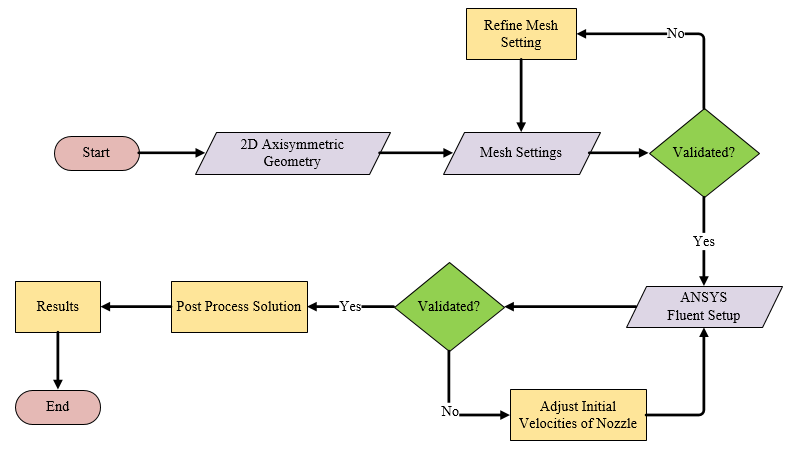
\includegraphics[height=0.45\textwidth]{images/SimulationProcessFlowChart.PNG}
    \label{fig:ejectorprocessflowchart}
\end{figure}
\end{frame}

\begin{frame}{2D Axisymmetric Model}
  \begin{figure}[h]
    \centering
    \includegraphics[width=1\textwidth]{images/ejectordrawing.png}
    \caption{Two Dimensional Axisymmetric Drawing of Ejector based from the 3D Geometry of Shah et al.\cite{shah2014experimental}}
    \label{fig:2daxisymmetricejector}
 \end{figure}
\end{frame}

\begin{frame}{Mesh Settings}
   \begin{figure}[h]
    \centering
    \includegraphics[width=0.5\textwidth]{images/Meshemphasized.png}
    \label{fig:meshrefinement1}
  \end{figure}
  \begin{table}[h]
      \centering
       \caption{Number of Elements and Nodes for Each Mesh Settings}
      \label{tab:meshelementsandnodes}
      \begin{tabular}{ccc}
      \hline
         Mesh Settings  &  Elements & Nodes\\
      \hline
         Refinement Level 1  & 87,412 & 178,106 \\
         Refinement Level 2 & 196,620 & 398,162 \\
         Refinement Level 3 & 349,496 & 705,554 \\
         Refinement Level 4 & 539,716 & 1,087,722 \\
      \hline
      \end{tabular}
  \end{table}
\end{frame}

\begin{frame}{Mesh Settings: Refinement Level 1}
  \begin{figure}[h]
    \centering
    \includegraphics[width=1\textwidth]{images/MeshRef1.png}
    \label{fig:meshrefinement1}
  \end{figure}
\end{frame}

\begin{frame}{Mesh Settings: Refinement Level 2}
    \begin{figure}[h]
    \centering
    \includegraphics[width=1\textwidth]{images/MeshRef2.png}
    \label{fig:meshrefinement2}
  \end{figure}
\end{frame}

\begin{frame}{Mesh Settings: Refinement Level 3}
    \begin{figure}[h]
    \centering
    \includegraphics[width=1\textwidth]{images/MeshRef3.PNG}
    \label{fig:meshrefinement3}
  \end{figure}
\end{frame}

\begin{frame}{Mesh Settings: Refinement Level 4}
    \begin{figure}[h]
    \centering
    \includegraphics[width=1\textwidth]{images/MeshRef4.PNG}
    \label{fig:meshrefinement4}
  \end{figure}
\end{frame}

\begin{frame}{Mesh Metrics and Computational Time}
    \begin{table}[h]
      \centering
       \caption{Mesh Metrics and Computational Time for Each Mesh Settings}
      \label{tab:meshelementsandnodes}
      \begin{tabular}{cccc}
      \hline
         Mesh Settings  & Orthogonal Quality  & Min. Aspect Ratio & Solving Time\\
      \hline
         Ref. Level 1  & 0.764862 & 3.32878 & 15 hours\\
         Ref. Level 2 & 0.751712 & 3.54955 & 70 hours\\
         Ref. Level 3 & 0.712621 & 3.48676 & 120 hours\\
         Ref. Level 4 & 0.816016 & 3.22583 & 170 hours\\
      \hline
      \end{tabular}
  \end{table}
\end{frame}

\begin{frame}{Mesh Independent Study:Static Pressure of the Mixture}
    \begin{figure}[h]
      \centering
      \includegraphics[height=5cm]{images/MISstaticpressure.png}
      \label{fig:meshindependentstudy}
   \end{figure}
\end{frame}

\begin{frame}{Mesh Independent Study: Pressure Coefficient and the Total Pressure}
    \begin{columns}
      \column{0.45\textwidth}
      \begin{figure}[h]
      \centering
      \includegraphics[height=4.5cm]{images/MISPCcalibrated.png}
      \label{fig:meshindependentstudy}
      \end{figure}
      \column{0.45\textwidth}
      \begin{figure}[h]
      \centering
      \includegraphics[height=4.5cm]{images/MISAbsP.png}
      \label{fig:meshindependentstudy}
      \end{figure}
    \end{columns}
\end{frame}

\begin{frame}{Mesh Independent Study: Dynamic Pressure}
       \begin{columns}
      \column{0.45\textwidth}
      \begin{figure}[h]
      \centering
      \includegraphics[height=4.5cm]{images/MISdynapair.png}
      \label{fig:meshindependentstudy}
      \end{figure}
      \column{0.45\textwidth}
      \begin{figure}[h]
      \centering
      \includegraphics[height=4.5cm]{images/MISdynapsteam.png}
      \label{fig:meshindependentstudy}
      \end{figure}
    \end{columns}
\end{frame}

\begin{frame}{Mesh Independent Study: Dynamic Pressure}
       \begin{columns}
      \column{0.45\textwidth}
      \begin{figure}[h]
      \centering
      \includegraphics[height=4.5cm]{images/MISdynapair.png}
      \label{fig:meshindependentstudy}
      \end{figure}
      \column{0.45\textwidth}
      \begin{figure}[h]
      \centering
      \includegraphics[height=4.5cm]{images/MISdynapwater.png}
      \label{fig:meshindependentstudy}
      \end{figure}
    \end{columns}
\end{frame}

\begin{frame}{Mesh Independent Study: Relative Total Pressure}
       \begin{columns}
      \column{0.45\textwidth}
      \begin{figure}[h]
      \centering
      \includegraphics[height=4.5cm]{images/MISRelTPAir.png}
      \label{fig:meshindependentstudy}
      \end{figure}
      \column{0.45\textwidth}
      \begin{figure}[h]
      \centering
      \includegraphics[height=4.5cm]{images/MISRTPsteam.png}
      \label{fig:meshindependentstudy}
      \end{figure}
    \end{columns}
\end{frame}

\begin{frame}{Mesh Independent Study: Relative Total Pressure}
       \begin{columns}
      \column{0.45\textwidth}
      \begin{figure}[h]
      \centering
      \includegraphics[height=4.5cm]{images/MISRelTPAir.png}
      \label{fig:meshindependentstudy}
      \end{figure}
      \column{0.45\textwidth}
      \begin{figure}[h]
      \centering
      \includegraphics[height=4.5cm]{images/MISRelTPwater.png}
      \label{fig:meshindependentstudy}
      \end{figure}
    \end{columns}
\end{frame}

\begin{frame}{Mesh Independent Study: Total Pressure}
       \begin{columns}
      \column{0.45\textwidth}
      \begin{figure}[h]
      \centering
      \includegraphics[height=4.5cm]{images/MISTPAir.png}
      \label{fig:meshindependentstudy}
      \end{figure}
      \column{0.45\textwidth}
      \begin{figure}[h]
      \centering
      \includegraphics[height=4.5cm]{images/MISTPsteam.png}
      \label{fig:meshindependentstudy}
      \end{figure}
    \end{columns}
\end{frame}

\begin{frame}{Mesh Independent Study: Total Pressure}
       \begin{columns}
      \column{0.45\textwidth}
      \begin{figure}[h]
      \centering
      \includegraphics[height=4.5cm]{images/MISTPAir.png}
      \label{fig:meshindependentstudy}
      \end{figure}
      \column{0.45\textwidth}
      \begin{figure}[h]
      \centering
      \includegraphics[height=4.5cm]{images/MISRelTPwater.png}
      \label{fig:meshindependentstudy}
      \end{figure}
    \end{columns}
\end{frame}

\begin{frame}{Computational Domain of the 2D Axisymmetric Ejector}
    \begin{table}[h]
    \centering
    \caption{Computational Domain of the 2D Axisymmetric Ejector using Refinement Level 3}
    \label{tab:computationaldomainejector}
    \begin{tabular}{ccc}
    \hline
        Domain Extents & Minimum (mm) & Maximum (mm) \\
    \hline
        x-coordinate &  -64.6339 & 245.3661 \\
        y-coordinate & 0.0000 & 15.325 \\
    \hline
    \end{tabular}
\end{table}
\end{frame}

\begin{frame}{Volume and Face Area Statistics of the 2D Axisymmetric Ejector using Refinement Level 3}
\begin{table}[h]
    \centering
    \caption{Volume Statistics}
    \label{tab:volumestat}
    \begin{tabular}{|c|c|}
      \hline
        Minimum volume (mm\textsuperscript3) &  0.002245853\\
     \hline
        Maximum volume (mm\textsuperscript3) & 0.8284871\\
     \hline
        Total volume (mm\textsuperscript3) & 104,100.4 \\
     \hline
        Minimum 2d volume (mm\textsuperscript3) & 2.593306 \\
     \hline
        Maximum 2d volume (mm\textsuperscript3) & 15.79421 \\
     \hline
    \end{tabular}
\end{table}
\begin{table}[h]
    \centering
    \caption{Face Area Statistics}
    \label{tab:faceareastat}
    \begin{tabular}{|c|c|}
       \hline
        Minimum face area (mm\textsuperscript2) & 50.53009  \\
       \hline
        Maximum face area (mm\textsuperscript2) & 162.0518 \\
       \hline
    \end{tabular}
\end{table}
\end{frame}

\begin{frame}{Material Properties: Stainless Steel AISI316}
    \begin{table}[h]
        \centering
        \begin{tabular}{|c|c|}
        \hline
            Density & 8,000 kg/m\textsuperscript{3} \\
        \hline
            Specific Heat & 500 J/kg K \\
        \hline
            Thermal Conductivity & 16.3 W/m K \\
        \hline
        \end{tabular}
        \label{tab:steelaiai316}
    \end{table}
\end{frame}
\begin{frame}{Fluid Properties: Steam Central Jet}
    \begin{table}[h]
        \centering
        \caption{Properties of Air}
        \label{tab:airprop}
        \begin{tabular}{|c|c|}
        \hline
            Density & 1.225 kg/m\textsuperscript{3}\\
        \hline
            Specific Heat & 1,006.43 J/kg K \\
        \hline
            Thermal Conductivity & 0.0242 W/m K \\
        \hline
            Viscosity & 1.7894e-05 kg/m-s \\
        \hline
            Molecular Weight & 28.966 kg/kmol \\
        \hline
            Standard State Enthalpy & 0 J/kg mol \\
        \hline
            Reference Temperature & 298.15 K \\
        \hline
        \end{tabular}
    \end{table}
\end{frame}

\begin{frame}{Fluid Properties: Steam Central Jet}
    \begin{table}[h]
        \centering
        \caption{Properties of Steam}
        \label{tab:steamprop}
        \begin{tabular}{|c|p{3cm}|}
        \hline
            Density  & $\rho = -31.14307 + 0.3099722 T - 0.00103197 T^{2} + 1.15e-06 T^{3}$\\
        \hline
            Specific Heat &  2121 J/kg K \\
        \hline
            Thermal Conductivity & 0.025506 W/m K \\
        \hline
            Viscosity & 1.2555e-05 kg/m-s \\
        \hline
            Molecular Weight & 18.01534 kg/kmol \\
        \hline
            Standard State Enthalpy & -2.418379e+08 J/kg mol \\
        \hline
            Reference Temperature & 298.15 K \\
        \hline
        \end{tabular}
    \end{table}
    Density varies from 280 to 400 K.
\end{frame}

\begin{frame}{Fluid Properties: Steam Central Jet}
    \begin{table}[h]
        \centering
        \caption{Properties of Water}
        \label{tab:waterprop}
        \begin{tabular}{|c|c|}
        \hline
            Density  & 998.8 kg/m\textsuperscript{3}\\
        \hline
            Specific Heat &  4186.6 J/kg K \\
        \hline
            Thermal Conductivity & 0.59229 W/m K \\
        \hline
            Viscosity & 0.001084 kg/m-s \\
        \hline
            Molecular Weight & 18.01534 kg/kmol \\
        \hline
            Standard State Enthalpy & -2.858412e+08 J/kg mol \\
        \hline
            Reference Temperature & 298.15 K \\
        \hline
        \end{tabular}
    \end{table}
\end{frame}

\begin{frame}{Boundary Conditions: Steam Central Jet}
\begin{table}[h]
    \centering
    \caption{Ejector Inlet Conditions}
    \label{tab:ejectorbc}
    \begin{tabular}{|c|c|}
    \hline
        Ejector & Water Inlet \\
    \hline
        Pressure Inlet & 93.56 kPa \\
    \hline
        Temperature Inlet & 290 K \\
    \hline
        Inlet Velocity & 31.73435 m/s \\
    \hline
    \end{tabular}
\end{table}
\begin{table}[h]
    \centering
    \caption{Nozzle Inlet Conditions}
    \label{tab:nozzlebc}
    \begin{tabular}{|c|c|}
    \hline
        Nozzle & Steam Inlet \\
    \hline
        Pressure Inlet & 140 kPa \\
    \hline
        Temperature Inlet & 382.44 K \\
    \hline
        Inlet Velocity & 0.75 m/s \\
    \hline
    \end{tabular}
\end{table}
\centering Ambient Pressure = 96 kPa
\end{frame}

\begin{frame}{Fluid Properties: Water Central Jet}
    \begin{table}[h]
        \centering
        \caption{Properties of Steam}
        \label{tab:steampropwcj}
        \begin{tabular}{|c|p{3cm}|}
        \hline
            Density  & $\rho = -7.6292 + 0.022047 T $\\
        \hline
            Specific Heat &  2071.1 J/kg K \\
        \hline
            Thermal Conductivity & 0.024352 W/m K \\
        \hline
            Viscosity & 1.2154e-05 kg/m-s \\
        \hline
            Molecular Weight & 18.01534 kg/kmol \\
        \hline
            Standard State Enthalpy & -2.418379e+08 J/kg mol \\
        \hline
            Reference Temperature & 298.15 K \\
        \hline
        \end{tabular}
    \end{table}
    Density varies from 370 to 385 K.
\end{frame}

\begin{frame}{Fluid Properties: Water Central Jet}
    \begin{table}[h]
        \centering
        \caption{Properties of Water}
        \label{tab:waterpropwcj}
        \begin{tabular}{|c|c|}
        \hline
            Density (Density varies from 370 to 385 K)  & $\rho = 1232.13 - 0.73368 T $\\
        \hline
            Specific Heat &  4227.4 J/kg K \\
        \hline
            Thermal Conductivity & 0.68017 W/m K \\
        \hline
            Viscosity & 0.00025636 kg/m-s \\
        \hline
            Molecular Weight & 18.01534 kg/kmol \\
        \hline
            Standard State Enthalpy & -2.858412e+08 J/kg mol \\
        \hline
            Reference Temperature & 298.15 K \\
        \hline
        \end{tabular}
    \end{table}
\end{frame}

\begin{frame}{CPU Specification}
    \begin{table}[]
        \centering
        \caption{Device Specification}
        \label{tab:devicespecification}
        \begin{tabular}{c|c}
            Processor &  Intel(R) Core(TM) i7-4700MQ CPU @ 2.40GHz   2.40 GHz\\
            Installed RAM & 16.0 GB (15.6 GB usable)\\
            System type & 64-bit operating system, x64-based processor \\
        \end{tabular}
    \end{table}
\end{frame}

\begin{frame}{CFD Models Used}
\begin{itemize}
    \item Eulerian Multiphase Model
    \item Explicit Volume Fraction Discretization
    \item Symmetric Model
    \item Two-Resistance Model
    \item Thermal-Phase Change Model
    \item Interfacial Area Concentration: Particle Method
    \item $\kappa-\varepsilon$ Realizable per Phase turbulence model
    \item Scalable Wall Function
\end{itemize}
\end{frame}

\begin{frame}{CFD Solution Methods and Controls}
    \begin{block}{Pressure-Velocity Coupling}
    Phase Coupled SIMPLE
    \end{block}
    \begin{block}{Spatial Discretization}
    Gradient Least Squares Cell Based
    \end{block}
    \begin{block}{Momentum, Turbulent Kinetic Energy, Turbulent Dissipation Rate and Energy}
    QUICK Scheme
    \end{block}
    \begin{block}{Volume Fraction}
    Modified HRIC
    \end{block}
\end{frame}

\begin{frame}{CFD Solution Monitors: Residual Errors}
  \begin{columns}
    \column{0.45\textwidth}
    \begin{table}[h]
        \centering
        \begin{tabular}{cc}
        \hline
            Residuals & Convergence Criterion \\
        \hline
            Continuity & 1e-08\\
            u-air & 1e-08\\
            u-steam & 1e-08\\
            u-water & 1e-08\\
            v-air & 1e-08\\
            v-steam & 1e-08\\
            v-water & 1e-08\\
        \hline
        \end{tabular}
    \end{table}
    \column{0.45\textwidth}
    \begin{table}[h]
        \centering
        \begin{tabular}{cc}
        \hline
            Residuals & Convergence Criterion \\
        \hline
            energy-p1 & 1e-08\\
            energy-p2 & 1e-08\\
            energy-p3 & 1e-08\\
            k-air & 1e-08\\
            k-steam & 1e-08\\
            k-water & 1e-08\\
            eps-air & 1e-08\\
            eps-steam & 1e-08\\
            eps-water & 1e-08\\
        \hline
        \end{tabular}
    \end{table}
  \end{columns}
\end{frame}

\section{Governing Equations and Solver Theory}
\begin{frame}{Eulerian Model: Conservation of Mass or Continuity Equation}
    \begin{equation} \label{gc2_eqn}
\frac{1}{\rho_r{}_q}(\frac{\partial}{\partial t }(\alpha_q\rho_q) + \nabla\cdot(\alpha_q\rho_q\vec{v_q})= \sum_{p=1}^{n} (\Dot{m_p{}_q}-\Dot{m_q{}_p}))
\end{equation}
where:\\
$\alpha_q = volume \:fraction \:of \:the \:q^{th} \:phase$\\
$\rho_q = density\:of \:the\: q^{th} \:phase$\\
$\vec{v_q} = velocity\: of\: the\: q^{th}\: phase$\\
$\Dot{m_p{}_q} = mass\: transfer\: from\: phase\: p\: to\: phase\: q$\\
$\Dot{m_q{}_p} = mass\: transfer\: from\: phase\: q\: to\: phase\: p\: $\\
\end{frame}

\begin{frame}{Eulerian Model: Conservation of Mass or Continuity Equation}
    The continuity equation or the volume fraction equation will not solved for the primary phase, the primary phase volume fraction will be computed based on the following constraint:\\
    \begin{equation}
        \sum_{p=1}^{n} \alpha_q = 1
    \end{equation}
    The volume fraction equation may be solved either through \textbf{Implicit} or \textbf{Explicit} \textbf{time discretization}. \textbf{Implicit} discretization is used for \textbf{stratified flows} while \textbf{Explicit} discretization is used for \textbf{jet flows}.
\end{frame}

\begin{frame}{Explicit Scheme: Volume Fraction Discretization Scheme}
    \begin{equation}
        \frac{\alpha_q^{n+1}\rho_q^{n+1}-\alpha_q^{n}\rho_q^{n}}{\Delta t}\:V \:+\:\sum_{f}(\rho_q U_f^{n}\alpha_{q,f}^{n})=\bigg[\sum_{p=1}^{n}(\Dot{m_p{}_q}-\Dot{m_q{}_p})\bigg]\:V
    \end{equation}
where:\\
$ n\:+\:1 = index \:for \:new \:(current) \:time \:step$\\
$ n = index\:for \:previous\: time \:step$\\
$\alpha_{q,f} = face\: value\: of\: q^{th}\: volume\: fraction,\: computed\: from\: the\: first-order\:or\:second-order\: upwind,\: QUICK,\: modified\: HRIC\:, or\: CICSAM\: scheme$\\
$V = volume\: of\: the\: cell$\\
$U_{f} = volume \: flux\: through\: the\: face,\: based\: on\: normal\: velocity\: $\\
\end{frame}

\begin{frame}{Eulerian Model: Conservation of Momentum}
    \begin{equation} \label{ffmansys_eqn}
    \begin{split}
    \frac{\partial}{\partial t }(\alpha_q\rho_q\vec{v_q}) 
    + \nabla\cdot(\alpha_q\rho_q\vec{v_q}\vec{v_q})
    = & -\alpha_q\nabla p + \nabla\cdot\Bar{\Bar{\tau_q}} 
    + \alpha_q\rho_q\vec{g} \\
    &+ \sum_{p=1}^{n} (K_p{}_q(\vec{v_p}-\vec{v_q}) + \Dot{m_p{}_q}\vec{v_p{}_q} - \Dot{m_q{}_p}\vec{v_q{}_p}) 
    \end{split}
\end{equation}
where:\\
$ \Bar{\Bar{\tau_q}}\: = stress-strain \:tensor \:of \:the \:q^{th} \:phase$\\
$ \vec{g} = acceleration\:due \:to\:gravity$\\
$K_p{}_q = mean\: interphase\: momentum\: exchange\: coefficient$\\
$\Dot{m_p{}_q} = interfacial\: mass\: transfer\: between\: p^{th}\: and\:q^{th}\:phase$\\
$\vec{v_p{}_q} = relative \: velocity\: of\: the\: p^{th}\: phase\: to\: the\: q^{th}\: phase $\\
$\vec{v_q{}_p} = relative \: velocity\: of\: the\: q^{th}\: phase\: to\: the\: p^{th}\: phase $\\
\end{frame}

\begin{frame}{Eulerian Model: Conservation of Energy}
    \begin{equation}\label{gcoe_eqn}
    \begin{split}
       \frac{\partial}{\partial t }(\alpha_q\rho_q h_q)
       &+ \nabla\cdot(\alpha_q\rho_q\vec{\mu_q} h_q)=\alpha_q\frac{\partial P_q}{\partial t}+\Bar{\Bar{\tau_q}}:\nabla\vec{\mu_q}-\nabla\cdot\vec{q_q}+ ... \\ &...+S_q+\sum_{p=1}^{n}(Q_p{}_q + \Dot{m_p{}_q} h_p{}_q - \Dot{m_q{}_p} h_q{}_p)
    \end{split}
\end{equation}
where:\\
$h_q = specific\: enthalpy\: of\: the\: q^{th}\:phase,\vec{q_q} = heat \: flux $\\
$S_q = source\: term\:that \: includes\:sources\:of\:enthalpy\:(By\:default\:S_q=0) $\\
$Q_{pq} = interfacial\:heat\:transfer $, $h_{pq} = interphase\:enthalpy$\\
The heat exchange between phases must comply with the local balance conditions: 
$Q_{pq}=-Q_{qp}\:and\:Q_{qq}=0 $\\
\end{frame}

\begin{frame}{Interfacial Area Concentration: Particle Method}
    \begin{equation}\label{satovr_eqn}
    A_p = \frac{\pi d_g^2}{\frac{1}{6}\pi d_g^3}=\frac{6}{d_g}
   \end{equation}
   \centering Particle Model
   \begin{equation} \label{iacm_eqn}
    A_f{}_g=\alpha_g A_p = \frac{6\alpha_g}{d_g}
   \end{equation}
where:\\
$A_p = area\:of\:the\:particle$\\
$d_g = diameter\:of\:the\:dispersed\:phase$\\
$A_{fg}= interfacial\:area\:concentration$\\
$\alpha_g = volume\:fraction\:of\:the\:dispersed\:phase$\\
\end{frame}

\begin{frame}{Interfacial Momentum Exchange Between Steam and Water}
    The exchange coefficient\:$K_f{}_g$ expresses in the following general equation as:
\begin{equation} \label{kfg_eqn}
    K_f{}_g = \frac{\rho_f{}_g f_d}{6 \tau_f{}_g} d_g A_f{}_g
\end{equation}
The particle relaxation time\: $\tau_f{}_g$ is generally expresses in the general equation as:
\begin{equation} \label{prt_eqn}
    \tau_f{}_g = \frac{\rho_f{}_g d_f{}_g^2}{18 \mu_f{}_g}
\end{equation}
where:\\
$\rho_{fg}=interfacial\:density,\mu_{fg}=interfacial\:viscosity, f_d = drag\:coefficient$\\ $d_{fg}=interfacial\:diameter$\\
\end{frame}

\begin{frame}{Interfacial Drag Model:Symmetric Model}
    \begin{equation} \label{rhofg_eqn}
    \rho_f{}_g = \alpha_f\rho_f + \alpha_g\rho_g
    \end{equation}
    \begin{equation} \label{mufg_eqn}
    \mu_f{}_g = \alpha_f\mu_f + \alpha_g\mu_g 
    \end{equation}
    \begin{equation} \label{dfg_eqn}
    d_f{}_g = \frac{1}{2} (d_f + d_g)
    \end{equation}
    \begin{equation}\label{kfgsym_eqn}
    K_f{}_g = \frac{\alpha_g(\alpha_f\rho_f+\alpha_g\rho_g)f_d}{\tau_f{}_g}
    \end{equation}
    \begin{equation}\label{taufgsym_eqn}
    \tau_f{}_g = \frac{(\alpha_f\rho_f+\alpha_g\rho_g) d_g^2}{18 (\alpha_f\mu_f + \alpha_g\mu_g)}
    \end{equation}
\end{frame}

\begin{frame}{Interfacial Heat Transfer Between Steam and Water}
    \begin{equation} \label{hq_eqn}
    h_q (T_q) = h (T_r{}_e{}_f) + \int_{T_r{}_e{}_f}^{T_q} C_p{}_,{}_q(T_q)\, dT_q
   \end{equation}
   \begin{equation} \label{hqs_eqn}
    h_q = \int C_p{}_,{}_q\, dT_q
  \end{equation}
  \centering Interfacial Volumetric Rate of Heat Transfer
  \begin{equation}\label{vht_eqn}
    Q_f{}_g = ht_f{}_g A_f{}_g (T_f-T_g)
  \end{equation}
\end{frame}

\begin{frame}{Two-Resistance Model}
\begin{columns}
    \column{0.45\textwidth}
    \begin{figure}
    \centering
    \includegraphics[height=5cm]{images/two resistance model.PNG}
    \caption{\centering Circuit diagram of a phasic volumes of steam and water and its interphase}
    \end{figure}
    \column{0.45\textwidth}
    \centering Interfacial Heat Transfer
    \begin{equation}\label{ihf_eqn}
    Q_g = -Q_f = ht_f{}_g A_f{}_g (T_f - T_g)
    \end{equation}
    \centering Interfacial Heat Transfer Coefficient
    \begin{equation}
    \frac{1}{ht_f{}_g} = \frac{1}{h_g} + \frac{1}{h_f}
    \end{equation}
    \begin{equation}
        ht_f{}_g = \frac{h_g h_f}{h_g + h_f}
    \end{equation}
\end{columns}
\end{frame}

\begin{frame}{Two-Resistance Model: Using Constants for Two-Resistors}
\begin{columns}
\column{0.45\textwidth}
Convective Heat Transfer Coefficient of Steam, $h_g$\cite{brucker1977direct,kosky2015exploring} 
\begin{align*}
    h_g = 10,000\:\frac{W}{m^{2}K}
\end{align*}
Convective Heat Transfer Coefficient of Water, $h_f$ \cite{kosky2015exploring,EngineeringToolbox}
\begin{align*}
    h_f = 1,000\:\frac{W}{m^{2}K}
\end{align*}
Free Convective Heat Transfer Coefficient of Air, $h_a$ \cite{kosky2015exploring}
\begin{align*}
    h_a = 25\:\frac{W}{m^{2}K}
\end{align*}
\column{0.45\textwidth}
Interfacial Heat Transfer Coefficient: 
\begin{itemize}
    \item Between Steam and Air
    \begin{align*}
        ht_g{}_a = \frac{10,000(25)}{10,000 + 25} = 24.938\frac{W}{m^{2}K}
    \end{align*}
    \item Between Water and Air
    \begin{align*}
        ht_w{}_a = \frac{1,000(25)}{1,000 + 25} = 24.390\frac{W}{m^{2}K}
    \end{align*}
    \item Between Steam and Water
    \begin{align*}
        ht_g{}_f = \frac{10,000(1,000)}{10,000 + 1,000} = 909.091\frac{W}{m^{2}K}
    \end{align*}
\end{itemize}
\end{columns}
\end{frame}

\begin{frame}{Interfacial Mass Transfer Between Steam and Water}
\begin{columns}
\column{0.45\textwidth}
\textbf{Thermal Phase Change Model:}
\begin{align*}
    \Dot{m_f{}_g} = \frac{ht_f A_f{}_g (T_s-T_f) + ht_g A_f{}_g (T_s - T_g)}{h_g{}_s - h_f{}_s}
    \end{align*}
    where:\\
    $h_{gs}$ and $h_{fs}$ are the phase enthalpies\\
    Note:\\
    Saturation Temperature ($T_{sat}$) is set to:
    \begin{align*}
        T_{sat} = 100^{\circ}C (373.15K)
    \end{align*}
\column{0.45\textwidth}
Condensation-Evaporation Model\cite{prakash1990two}\\
If $\Dot{m_f{}_g}\ge0$ (evaporation):
\begin{align*}
    h_f{}_s &= h_f(T_f)\\
    h_g{}_s &= h_g(T_{sat}) = 2,675.6 kJ/kg
\end{align*}
If $\Dot{m_f{}_g}<0$ (condensation):
\begin{align*}
    h_f{}_s &= h_f(T_{sat}) = 419.17 kJ/kg\\
    h_g{}_s &= h_g(T_{g})
\end{align*}
Latent Heat (L):
\begin{align*}
    L = h_{g}(T_{sat})-h_{f}(T_{sat}) = 2,256.43 kJ/kg
\end{align*}
\end{columns}
\end{frame}

\begin{frame}{Turbulence Model: Transport Equations for the Realizable \boldmath{$\kappa-\varepsilon$} model}\label{Rkvarepsilon_par}
    \begin{equation}\label{Rkappa_eqn}
    \frac{\partial}{\partial t} (\rho \kappa) + \frac{\partial}{\partial x_j}\big(\rho \kappa u_j\big) = \frac{\partial}{\partial x_j}\bigg[\Big(\mu + \frac{\mu_t}{\sigma_\kappa}\Big)\frac{\partial \kappa}{\partial x_j}\bigg] + G_\kappa + G_b -\rho\varepsilon-Y_M+S_\kappa
    \end{equation}
    \begin{equation}\label{Repsilon_eqn}
    \begin{split}
    \frac{\partial}{\partial}(\rho \varepsilon) 
    & + \frac{\partial}{\partial x_j}\big(\rho \varepsilon u_j\big) = \frac{\partial}{\partial x_j}\bigg[\Big(\mu + \frac{\mu_t}{\sigma_\varepsilon}\Big)\frac{\partial \varepsilon}{\partial x_j}\bigg]+ ... \\
    &... + \rho C_1 S_\varepsilon - \rho C_2 \frac{\varepsilon^2}{\kappa + \sqrt{\nu \varepsilon}} + C_1{}_\varepsilon \frac{\varepsilon}{\kappa} C_3{}_\varepsilon G_b + S_\varepsilon
    \end{split}
   \end{equation}
where,
\begin{equation}\label{C1_eqn}
    C_1 = max \bigg [0.43, \frac{\eta}{\eta + 5}\bigg], \eta = S\frac{\kappa}{\varepsilon}, S = \sqrt{2 S_i{}_j S_i{}_j}
\end{equation}
\end{frame}

\begin{frame}{Multiphase \boldmath{$\kappa-\varepsilon$} Turbulence Model for Each Phase}
    \begin{equation} \label{Rkappamulti_eqn}
    \begin{split}
    & \frac{\partial}{\partial t}\Big(\alpha_q\rho_q\kappa_q\Big) 
    + \nabla\cdot\Big(\alpha_q\rho_q \vec{U_q}\kappa_q\Big) = \\
    & \nabla\cdot\Bigg(\alpha_q\bigg(\mu_q + \frac{\mu_{t,q}}{\sigma_\kappa}\bigg)\nabla \kappa_q\Bigg) + \Big(\alpha_q G_{\kappa,q} - \alpha_q\rho_q\varepsilon_q\Big) +\dotsm \\
    &\dotsm + \sum_{p=1}^{N} K_{pq}\Big(C_{pq}\kappa_p - C_{qp}\kappa_q\Big) - \sum_{p=1}^{N} K_{pq} \Big(\vec{U_p}-\vec{U_q}\Big)\cdot\frac{\mu_{t,p}}{\alpha_p \sigma_p}\nabla \alpha_p +\dotsm \\
    &\dotsm + \sum_{p=1}^{N} K_{pq} \Big(\vec{U_p}-\vec{U_q}\Big)\cdot\frac{\mu_{t,q}}{\alpha_q \sigma_q}\nabla \alpha_q + \prod \kappa_q + \prod \kappa_p
    \end{split}
\end{equation}
\end{frame}

\begin{frame}{Multiphase \boldmath{$\kappa-\varepsilon$} Turbulence Model for Each Phase}
    \begin{equation}\label{Repsilonmulti_eqn}
    \begin{split}
      & \frac{\partial}{\partial t} \Big(\alpha_q\rho_q\varepsilon_q\Big) + \nabla\cdot\Big(\alpha_q\rho_q \vec{U_q}\varepsilon_q\Big) = \\ 
       & \nabla\cdot\Bigg(\alpha_q\bigg(\mu_q + \frac{\mu_{t,q}}{\sigma_\varepsilon}\bigg)\nabla \varepsilon_q\Bigg) + \alpha_q\rho_q C_{1\varepsilon} S_{k,q} \varepsilon_q - \alpha_q\rho_q C_{2\varepsilon} \frac{\varepsilon_q^2}{k_q + \sqrt{\nu_q \varepsilon_q}}+\dotsm \\
       &\dotsm + C_{3\varepsilon}\frac{\varepsilon_q}{\kappa_q}\bigg[\sum_{p=1}^{N} K_{pq}\Big(C_{pq}\kappa_p - C_{qp}\kappa_q\Big) - \sum_{p=1}^{N} K_{pq} \Big(\vec{U_p}-\vec{U_q}\Big)\cdot\frac{\mu_{t,p}}{\alpha_p \sigma_p}\nabla \alpha_p \\
      & + \sum_{p=1}^{N} K_{pq} \Big(\vec{U_p}-\vec{U_q}\Big)\cdot\frac{\mu_{t,q}}{\alpha_q \sigma_q}\nabla \alpha_q\bigg] + \prod \varepsilon_r
    \end{split}
\end{equation}
\end{frame}

\begin{frame}{Steam Equation of State\cite{ansys2011ansys}}
Steam Equation of State that relates the pressure (P) to the vapor density $\rho_{v}$ and the temperature (T) by a virial equation\cite{young1988equation},
    \begin{equation}
        P = \rho_{v}RT (1 + B\rho_{v} + C\rho_{v}^{2})
    \end{equation}
where B and C are the second and the third virial coefficients given the following empirical equations:
    \begin{equation}
        B = a_{1}(1 + \frac{\tau}{\alpha})^{-1} + a_{2}e^{\tau}(1 - e^{-\tau})^{\frac{5}{2}} + a_{3}\tau
    \end{equation}
where B is given in $\frac{m^{3}}{kg}$, $\tau=\frac{1500}{T}$, with T given in Kelvin (K)
\end{frame}

\begin{frame}{Steam Equation of State\cite{ansys2011ansys}}
        $\alpha = 10000.0, a_{1} = 0.0015, a_{2} = -0.000942, and a_{3} = -0.0004882$
    \begin{equation}
        C = a (\tau - \tau_{o})e^{-\alpha \tau} + b
    \end{equation}
where C is given in $\frac{m^{6}}{kg^{2}}$, $\tau = \frac{T}{647.286}$ with T given Kelvin, $\tau_{o}=0.8978$, $\alpha=11.16$, $a=1.772$ and $b=1.5e^{-06}$.\\
The two empirical functions that define the virial coefficients $B$ and $C$ cover the temperature range from 273 K to 1073 K.
\end{frame}

\begin{frame}{Steam Equation of State\cite{ansys2011ansys}}
    The vapor isobaric specific heat capacity $Cp_{v}$ is given by:
    \begin{equation}
       \begin{split}
           Cp_{v} = & Cp_{o}(T) 
                      \\ 
                    & + R[[(1-\alpha_{v}T)(B-B_{1})-B_{2}]\rho_{v}] \\
                    & + [(1-2\alpha_{v}T)C+\alpha_{v}TC_{1}-\frac{C_{2}}{2}]\rho_{v}^2] \\
       \end{split}
    \end{equation}
    where $Cp_{o}$ is in $\frac{kJ}{kg-K}$, and, \\
    $B_{1} = T \frac{dB}{dT}, C_{1} = T\frac{dC}{dT}, B_{2} = T^{2}\frac{dB^{2}}{dT^{2}}$, and $C_2 = T^{2} \frac{dC^{2}}{dT^{2}}$.
\end{frame}

\begin{frame}{Steam Equation of State\cite{ansys2011ansys}}
The vapor specific enthalpy, $h_{v}$ is given by:
    \begin{equation}
        h_{v} = h_{o}(T) + RT[(B - B_{1})\rho_{v} + (C-\frac{C_{1}}{2})\rho_{v}^2]
    \end{equation}
The vapor specific entropy, $s_{v}$ is given by:
    \begin{equation}
        s_{v} = s_{o}(T) + R[(B - B_{1})\rho_{v} + \frac{(C+{C_{1}})}{2}\rho_{v}^2]
    \end{equation}
\end{frame}

\begin{frame}{Steam Equation of State\cite{ansys2011ansys}}
    The isobaric specific heat at zero pressure is defined by the following empirical equation:
    \begin{equation}
        Cp_{o}(T) = \sum_{i=1}^{6} a_{i}T^{i-2}
    \end{equation}
    where $Cp_{o}$ is in $\frac{kJ}{kg-K}$, $a_{1}=46.0$,$a_{2}=1.47276$, $a_{3}=8.38930e-04$,$a_{4}=-2.19989e-07$, $a_{5}=2.46619e-10$, and $a_{6}=-9.70466e-14$.
\end{frame}

\begin{frame}{Steam Equation of State\cite{ansys2011ansys}}
    Both $h_{o}(T)$ and $s_{o}(T)$ are functions of temperature and they are defined by:
    \begin{equation}
        h_{o}(T) = \int Cp_{o} \,dT + h_{c}
    \end{equation}
    \begin{equation}
        s_{o}(T) = \int \frac{Cp_{o}}{T} \,dT + s_{c}
    \end{equation}
    where $h_{c}$ and $s_{c}$ are arbitrary constants.\\
    The vapor dynamic viscosity $\mu_{v}$ and thermal conductivity $k_{v}$ are also functions of temperature and were obtained from the journal entitled "The spontaneous condensation of steam in supersonic nozzles" by J.B. Young 1982\cite{young1982spontaneous}.
\end{frame}

\begin{frame}{T-s diagram showing the range of application of the equation of state\cite{young1988equation}}
    \begin{figure}
        \centering
        \includegraphics[height=5cm]{images/tsdiagramrangeofapplicationeos.jpg}
    \end{figure}
\end{frame}

\begin{frame}{Scalable Wall Functions\cite{ansys2017ansys}}
    The purpose of the scalable wall functions is to force the usage of the log law in conjunction with the standard wall functions approach. This is achieved by introducing a limiter in the y* calculations such that:
    \begin{equation}
        \tilde{y^*} = MAX(y^*, y_{limit}^*)
    \end{equation}
    where:\\
        $y_{limit}^* = 11.225.$\\
    The context of the scalable wall function is straightforward, thus, the \textbf{y* formulation used for any standard wall function is replaced by $\tilde{y^*}$.}
\end{frame}

\begin{frame}{Standard Wall Functions: Momentum Equation\cite{ansys2017ansys}}
\begin{columns}
  \column{0.45\textwidth}
    Law-of-the-wall for the dimensionless mean velocity yields:
  \begin{align*}
    U^* &= \frac{1}{\kappa}ln(Ey^*)\\
    U^* &\equiv U_p C_{\mu}^\frac{1}{4} k_p^\frac{1}{2} 
  \end{align*}
  The dimensionless distance from the wall expressed as:
  \begin{equation}
      y^* \equiv \frac{\rho C_{\mu}^\frac{1}{4} k_p^\frac{1}{2} y_p}{\mu}
  \end{equation}
  \scriptsize Note: Logarithmic law for the mean velocity is known to be valid for $30<y^*<300$, log-law is employed when $y^*>11.225$. When $y^*<11.225, U^*=y^*$.
  \column{0.45\textwidth}
  where:\\
  $\kappa = von\: Karmann\:constant\:(=0.4187)$ \\
  $E = empirical\:constant\:(9.793)$ \\
  $U_{p} = mean\:velocity\:of\:the\:fluid\:at\:the\:near-wall\:node\:P$ \\
  $k_p = turbulence\:kinetic\:energy\:at\:the\: near-wall\:node\:P$\\
  $y_p = distance\:from\:point\:P\:to\:the\:wall$\\
  $\mu = dynamic\:viscosity\:of\:the\:fluid$\\
  \scriptsize Note: In ANSYS Fluent, laws-of-the-wall for mean velocity and temperature are based on the wall unit,$y^*$, rather than $y^+ (\equiv \frac{\rho u_{\tau} y}{\mu})$. These quantities are approximately equal in equilibrium turbulent boundary layers.
\end{columns}
\end{frame}

\begin{frame}{Standard Wall Functions: Energy Equation\cite{ansys2017ansys}}
    \begin{equation*}
     T^* \equiv \frac{(T_w - T_p)\rho C_p k_p^\frac{1}{2}}{\Dot{q}} = \left\{
        \begin{array}{ll}
            Pry^* + \frac{1}{2} \rho Pr \frac{C_\mu^\frac{1}{4}k_p^\frac{1}{2}}{\Dot{q}} U_p^2 & \quad y^* < y_T^* \\
            Pr_t[\frac{1}{\kappa}ln(Ey^*)+\rho]+\cdots \\
            \cdots + \frac{1}{2} \rho Pr \frac{C_\mu^\frac{1}{4}k_p^\frac{1}{2}}{\Dot{q}}[Pr_tU_p^2 + (Pr-Pr_t)U_c^2]  & \quad y^* > y_T^* 
        \end{array}
    \right.
    \end{equation*}
  where P is computed as:
    \begin{equation}
        P = 9.24 \bigg[\bigg(\frac{Pr}{Pr_t}\bigg)^\frac{3}{4}-1\bigg]\bigg[1 + 0.28e^\frac{-0.007Pr}{Pr_t}\bigg]
    \end{equation}
    \label{stdwallfuncenergyeqn}
\end{frame}

\begin{frame}{Standard Wall Functions: Energy Equation}
    In slide \ref{stdwallfuncenergyeqn}:\\
    $k_p = turbulent\:kinetic\:energy\:at\:the\:first near-wall\:node\:P$\\
    $\rho = density\:of\:the\:fluid$\\
    $C_p = specific\:heat\:of\:fluid$\\
    $\Dot{q}= wall\:heat\: flux$\\
    $T_p = temperature\:at\:the\:first\:near-wall\:node\:P$\\
    $T_w = temperature\:at\:the\:wall$\\
    $Pr = molecular\:Prandtl\:number\:(\mu C_p/k_f)$\\
    $Pr_t = turbulent\:Prandtl\:number(0.85\:at\:the\:wall)$\\
    $U_c = mean\:velocity\:magnitude\:at\:y^*=y_T^*$
\end{frame}

\begin{frame}{Heat Transfer Coefficient for $CO_2$: Hughmark Model}
    \begin{equation*}
     Nu_p  = \left\{
        \begin{array}{lll}
            2 + 0.6 Re_p^\frac{1}{2} Pr^\frac{1}{3} & \quad 0\leq Re_p < 776.06 & \quad 0\leq Pr < 250 \\
            2 + 0.27 Re_p^{0.62} Pr^\frac{1}{3}  & \quad 776.06\leq Re_p  & \quad 0\leq Pr < 250
        \end{array}
    \right.
    \end{equation*}
    \begin{equation*}
        h_p = \frac{k_p Nu_p}{d_g}
    \end{equation*}
    where:\\
    $Nu_p = Nusselt\:number\:of\:the\:p^{th}\:phase$\\
    $Re = Reynolds\:number\:of\:the\:p^{th}\:phase$\\
    $Pr = Prandtl\:number$\\
    $h_p = heat\:transfer\:coefficient\:of\:the\:p^{th}\:phase,$\\
    $k_p = thermal\:conductivity\:of\:the\:p^{th}\:phase, d_g = particle\:diameter$
\end{frame}

\section{Validation of the CFD Model}
\begin{frame}{Validation of 2D Axisymmetric model:Two-Phase Steam Ejector}
    \begin{figure}
        \centering
        \includegraphics[height=5.25cm]{images/ValidationPressureProfile.jpg}
        \label{fig:shahexperimental}
    \end{figure}
\end{frame}

\begin{frame}{Two-Phase Steam Ejector}
    \begin{columns}
  \column{0.45\textwidth}
    \begin{figure}
        \centering
        \includegraphics[height=4.5cm]{images/tpseprescoef.png}
    \end{figure}
  \column{0.45\textwidth}
  \begin{figure}
        \centering
        \includegraphics[height=4.5cm]{images/tpseabspres.png}
    \end{figure}
 \end{columns}
\end{frame}

\begin{frame}{Two-Phase Steam Ejector}
    \begin{columns}
  \column{0.45\textwidth}
    \begin{figure}
        \centering
        \includegraphics[height=4.5cm]{images/tpseRTPsteam.png}
    \end{figure}
  \column{0.45\textwidth}
  \begin{figure}
        \centering
        \includegraphics[height=4.5cm]{images/tpsetpsteam.png}
    \end{figure}
 \end{columns}
\end{frame}

\begin{frame}{Two-Phase Steam Ejector}
    \begin{columns}
  \column{0.45\textwidth}
    \begin{figure}
        \centering
        \includegraphics[height=4.5cm]{images/tpsertpwater.png}
    \end{figure}
  \column{0.45\textwidth}
  \begin{figure}
        \centering
        \includegraphics[height=4.5cm]{images/tpsetpwater.png}
    \end{figure}
 \end{columns}
\end{frame}

\begin{frame}{Validation of 2D Axisymmetric model: Two-Phase CO2 Converging-Diverging Nozzle: Mixture of CO2 and Air}
 \begin{columns}
  \column{0.45\textwidth}
    \begin{figure}
        \centering
        \includegraphics[height=4.5cm]{images/co2718secresult.png}
        \caption{Time Step of 0.000718 sec}
    \end{figure}
  \column{0.45\textwidth}
  \begin{figure}
        \centering
        \includegraphics[height=4.5cm]{images/co2at135sec.png}
        \caption{Time Step of 0.00113 sec (Steady Operation)}
    \end{figure}
 \end{columns}
\end{frame}

\begin{frame}{Validation of 2D Axisymmetric model: Two-Phase CO2 Converging-Diverging Nozzle:Air and CO2}
 \begin{columns}
  \column{0.45\textwidth}
    \begin{figure}
        \centering
        \includegraphics[height=4.5cm]{images/cdnco2totalpress.png}
    \end{figure}
  \column{0.45\textwidth}
  \begin{figure}
        \centering
        \includegraphics[height=4.5cm]{images/cdnco2press1.png}
    \end{figure}
 \end{columns}
\end{frame}

\begin{frame}{Validation of 2D Axisymmetric model: Two-Phase CO2 Converging-Diverging Nozzle:Air and CO2}
 \begin{columns}
  \column{0.45\textwidth}
    \begin{figure}
        \centering
        \includegraphics[height=4.5cm]{images/cdnrelativepress1.png}
    \end{figure}
  \column{0.45\textwidth}
  \begin{figure}
        \centering
        \includegraphics[height=4.5cm]{images/cdnrelativepress2.png}
    \end{figure}
 \end{columns}
\end{frame}

\begin{frame}{Validation of 2D Axisymmetric model: Two-Phase CO2 Converging-Diverging Nozzle: Air and CO2}
 \begin{columns}
  \column{0.45\textwidth}
    \begin{figure}
        \centering
        \includegraphics[height=4.5cm]{images/co2dynamicpressair.png}
    \end{figure}
  \column{0.45\textwidth}
  \begin{figure}
        \centering
        \includegraphics[height=4.5cm]{images/co2dynamicpres.png}
    \end{figure}
 \end{columns}
\end{frame}

\section{Results and Discussion}
\begin{frame}{Pressure Contours on Steam Central Jet}
    \begin{figure}
        \centering
        \label{fig:pressurecontoursmeshref3}
        \includegraphics[height=5cm]{images/PressureContour.PNG}
    \end{figure}
\end{frame}

\begin{frame}{Pressure Plot on Steam Central Jet}
   \begin{figure}
    \centering
    \label{fig:pressureplot}
    \includegraphics[height=5cm]{images/PressurePlot.jpg}
   \end{figure}
\end{frame}

\begin{frame}{Velocity Contours on Steam Central Jet}
    \begin{figure}
        \centering
        \includegraphics[height=5cm]{images/sjcentralairvel.png}
    \end{figure}
\end{frame}

\begin{frame}{Velocity Contours on Steam Central Jet}
    \begin{figure}
        \centering
        \includegraphics[height=5cm]{images/sjcentralsteamvel.png}
    \end{figure}
\end{frame}

\begin{frame}{Velocity Contours on Steam Central Jet}
    \begin{figure}
        \centering
        \includegraphics[height=5cm]{images/sjcentralwatervel.png}
    \end{figure}
\end{frame}

\begin{frame}{XY Plots on Steam Central Jet}
  \begin{columns}
   \column{0.45\textwidth}
   \begin{figure}
    \centering
    \label{fig:velocityplot}
    \includegraphics[height=4.5cm]{images/velocityplotcorrect.png}
   \end{figure}
   \column{0.45\textwidth}
   \begin{figure}
        \centering
        \includegraphics[height=4.5cm]{images/temperatureprofile.jpg}
        \label{fig:axial temperature plot}
    \end{figure}
  \end{columns}
\end{frame}

\begin{frame}{Y Plus on Steam Central Jet}
  \begin{columns}
   \column{0.45\textwidth}
   \begin{figure}
    \centering
    \includegraphics[height=4.5cm]{images/EjectorWallYplus.jpg}
   \end{figure}
   \column{0.45\textwidth}
   \begin{figure}
    \centering
    \includegraphics[height=4.5cm]{images/nozzlewallyplus.jpg}
   \end{figure}
  \end{columns}
\end{frame}

\begin{frame}{Water Central Jet: Pressure Plot}
   \begin{columns}
   \column{0.45\textwidth}
   \begin{figure}
    \centering
    \includegraphics[height=4.5cm]{images/wcwfluids.png}
   \end{figure}
   \column{0.45\textwidth}
   \begin{figure}
    \centering
    \includegraphics[height=4.5cm]{images/wcandsc.png}
   \end{figure}
  \end{columns}
\end{frame}

\begin{frame}{Water Central Jet: Pressure Contour}
    \begin{figure}
        \centering
        \includegraphics[height=4.25cm]{images/wcpressureplot.png}
    \end{figure}
\end{frame}

\begin{frame}{Water Central Jet: Velocity Plot}
    \begin{figure}
        \centering
        \includegraphics[height=5.5cm]{images/wcjetvelocity.png}
    \end{figure}
\end{frame}

\begin{frame}{Water Central Jet: Velocity Contours}
    \begin{figure}
        \centering
        \includegraphics[height=5.5cm]{images/wcvelocityair.png}
    \end{figure}
\end{frame}

\begin{frame}{Water Central Jet: Velocity Contours}
    \begin{figure}
        \centering
        \includegraphics[height=5.5cm]{images/wcjetwatervelcon.png}
    \end{figure}
\end{frame}

\begin{frame}{Water Central Jet: Velocity Contours}
    \begin{figure}
        \centering
        \includegraphics[height=5.5cm]{images/wcjetsteamvelcon.png}
    \end{figure}
\end{frame}

\begin{frame}{Water Central Jet: Axial Temperature Distribution}
    \begin{figure}
        \centering
        \includegraphics[height=5.5cm]{images/wcjetaxialtemp.png}
    \end{figure}
\end{frame}

\begin{frame}{Y Plus on Water Central Jet}
  \begin{columns}
    \column{0.45\textwidth}
    \begin{figure}
        \includegraphics[height=4.5cm]{images/wcjetnozyplus.png}
    \end{figure}
    \column{0.45\textwidth}
    \begin{figure}
        \includegraphics[height=4.5cm]{images/wcjetejecyplus.png}
    \end{figure}
  \end{columns}
\end{frame}

\begin{frame}{Partial Evaporation of Water Central Jet:20\% vapor quality}
\begin{columns}
    \column{0.45\textwidth}
        \begin{figure}
        \centering
        \includegraphics[height=4.5cm]{images/partialevap20percent.png}
    \end{figure}
    \column{0.45\textwidth}
        \begin{figure}
        \centering
        \includegraphics[height=4.5cm]{images/pevaperprinitial1.png}
    \end{figure}
\end{columns}
\end{frame}

\begin{frame}{Partial Evaporation of Water Central Jet:20\% vapor quality}
\begin{columns}
    \column{0.45\textwidth}
        \begin{figure}
        \centering
        \includegraphics[height=4.5cm]{images/pe20vqver.png}
    \end{figure}
    \column{0.45\textwidth}
        \begin{figure}
        \centering
        \includegraphics[height=4.5cm]{images/pe20vqerpr.png}
    \end{figure}
\end{columns}
\end{frame}

\begin{frame}{Partial Evaporation of Water Central Jet:20\% vapor quality}
  \begin{columns}
    \column{0.45\textwidth}
    \begin{figure}
        \centering
        \includegraphics[height=4.5cm]{images/pe20vqpdvser.png}
    \end{figure}
    \column{0.45\textwidth}
    \begin{figure}
        \centering
        \includegraphics[height=4.5cm]{images/pe20vqpercentincpr.png}
    \end{figure}
  \end{columns}
\end{frame}

\begin{frame}{Initial Findings of the Study}
    \begin{itemize}
        \item The Water Central Jet has pressure drop along the entry of the nozzle and throat mixing area because of the effects of cavitation.
        \item On the Effects of Partial Evaporation, the introducing of vapor to the motive fluid increases the pressure recovery (i.e. pressure ratio) of the ejector, however, further increasing the Entrainment Ratio leads to decrease of pressure recovery because of the pressure drift loss of the secondary fluid to the induced vapor of the motive steam.
    \end{itemize}
\end{frame}

\begin{frame}{Expectations from the Completion of this Research}
    \begin{itemize}
        \item Comprehensive Characterization of the Ejector thru its sensitivity analysis by varying its Ejector Area Ratio, Entrainment Ratio, and Vapor Quality.
        \item Conduct Thermodynamic Analysis to the NOHTFPECGPPIE, this includes exergy analysis, UA analysis, etc.
    \end{itemize}
\end{frame}

\section{Timeline of Activities and Proposal Budget}
\begin{frame}{Gantt Chart (Research Plan)}
    \begin{figure}
        \centering
        \includegraphics[height=0.25\textwidth]{images/ganttchart2.png}
    \end{figure}
\end{frame}

\begin{frame}{Items for Reimbursement}
    \begin{table}[]
        \centering
        \begin{tabular}{ccc}
        \hline
            Hardwares and Softwares & Quantity &  Price\\
        \hline
            HP 15” Z Book Mobile Workstation & 1 & P127, 046.86 \\
            NIST REFPROP Software & 1 & P17,785.23 \\
            Visio Software Monthly Subscription & 1 & P20,000 \\
            OverLeaf LaTEX Monthly Subscription & 1 & P5,000 \\
            Minitab 6-Months Subscription & 1 & P1,500 \\
        \hline
           Total & 5 & P171,332.09 \\
        \hline
        \end{tabular}
    \end{table}
\end{frame}

\begin{frame}{Items for Reimbursement: Remote Learning and Zoom Meeting}
    \begin{table}[h]
        \centering
        \begin{tabular}{ccc}
        \hline
            Accessories and Devices  & Quantity &  Price\\
        \hline
            GLOBE Unli Fiber Plan 1899 Monthly Subscription & 1 & P8,000 \\
            Headset & 1 & P300 \\
            Camera and Ring Light & 1 & P500 \\
            Condensible Microphone & 1 & P300 \\
            edX LaTEX e-course & 1 & 3,500 \\
        \hline
            Total & 5 & P12,600 \\
        \hline
        \end{tabular}
    \end{table}
\end{frame}

\begin{frame}{Items to Purchase}
    \begin{table}[h]
        \centering
        \begin{tabular}{ccc}
        \hline
            Hardware and Software & Quantity & Price  \\
        \hline
            HP All-In-One Desktop & 1 & P100,00\\
            EES Software & 1 & P60,000 \\
            EES Self-Tutorial Manual & 1 &P3,000\\
         \hline 
            Total & 3 & P163,000 \\
         \hline
        \end{tabular}
    \end{table}
\end{frame}

\section{References}
\begin{frame}[allowframebreaks]
    \frametitle{References}
    \bibliographystyle{ieeetr}
    \bibliography{references}
\end{frame}
    
\section{References}

\end{document}
